\section{The Structural Approach to Auction Data}\label{sec:15-approach}

This section sets up the framework that the rest of the chapter uses. It defines the primitives and the
observables, states the sampling assumptions, gives precise definitions of identification and testability, and
previews the two broad estimation strategies that the later sections develop.

Auctions suit this program for the reasons given in \cref{sec:14-why-data}. Bids, prices, the number of bidders
and often the identities of the bidders are recorded. Above all, the seller writes down the rules, so the mapping
from bids to the allocation and to payments is known to the researcher. \citet[Section~1]{AtheyHaile2007} observe
that the primitives of any strategic model are the players, the information structure, the rules of play and the
players' objectives. In auction markets these elements can be described with unusual confidence. The only
behavioral assumption left is equilibrium play.

The structural approach targets questions that bids alone cannot answer. \citet[Section~1]{AtheyHaile2007} list
several. Some concern the division of rents in auctions of public resources, the adequacy of reserve prices in
government auctions, and the effects of mergers between bidders on procurement costs. The last is a merger
simulation of the kind studied in \cref{ch:mergers}, with the advantage that the game form is known. Others concern the
revenue consequences of changing the auction rules, the efficiency of bundling procurement contracts and the value
of seller reputations. Still others concern information-acquisition costs, adverse selection created by private
information, and risk aversion. Each question needs the distribution functions that describe bidders' demand and information. They
add a methodological point. Economic theory shapes many parts of an empirical model, but it rarely says anything
about the distributions of unobservables. Much of what auction data can teach us does not depend on such
distributional assumptions \citep[Section~1]{AtheyHaile2007}.

\subsection{Primitives and observables}\label{sec:15-primitives}

A single indivisible object is sold to one of $n\ge2$ risk-neutral bidders. Bidder $i$ has a value $V_i$ for the
object and private information summarized by a signal $S_i$. Upper-case letters denote random variables and
lower-case letters their realizations. The general model of \cref{sec:14-info} specifies the joint distribution of
values and signals. The two classes of models in \cref{def:14-private-values} differ in whether a rival's signal
is informative about one's own value. In a \emph{private values} (PV) model it is not, and we normalize $S_i=V_i$.
The primitive is then the joint distribution $F_{\bm V}$ of the vector of values $\bm V=(V_1,\dots,V_n)$. In the
\emph{independent private values} (IPV) model, $F_{\bm V}(\bm v)=\prod_{i=1}^nF_i(v_i)$. In the \emph{symmetric}
IPV model (SIPV), every $F_i$ equals a common $F$ with density $f$. In a \emph{common values} (CV) model a bidder
would revise her expected value if she learned a rival's signal \citep[p.~2110]{AtheyHaile2002}. Its primitive is
the joint distribution of values and signals.

We maintain the setting of \citet[Section~2.1]{AtheyHaile2002} unless a section says otherwise. The number of
bidders is common knowledge and there is no reserve price. Bidders play a Bayesian Nash equilibrium in weakly
undominated strategies, symmetric when bidders are symmetric. Ascending auctions follow the button model of
\cref{def:14-button}, in which bidders exit observably and irrevocably as the price rises.

The data never contain values. \citet[Section~2.2]{AtheyHaile2002} distinguish what is always observed from what is
sometimes observed. The econometrician always sees the number of bidders $n_t$ and the transaction price $P_t$ of
each auction $t$. With asymmetric bidders, the set of participants is also known. The following may or may not be
available:
\begin{enumerate}[label=(\roman*)]
\item bids other than the transaction price,
\item bidder identities, in particular the identity $I_t$ of the winner,
\item \emph{auction covariates} $Z_t$, such as the appraised value of the object or its realized ex post value,
\item \emph{bidder covariates} $W_{it}$, such as firm size, location, distance to the project or backlog.
\end{enumerate}
The format determines which bids exist. A sealed-bid auction can record every bid. A Dutch auction stops at the
first bid, so only the winning bid exists. An ascending auction ends when the next-to-last bidder drops out, so the
price at which the winner would have exited is never revealed (\cref{sec:14-spa-data}).

A last type of information is variation in the number of bidders. Participation is \emph{exogenous} if the joint
distribution of the signals of any subset of bidders does not depend on which other bidders participate
\citep[p.~2113]{AtheyHaile2002}. Exogenous variation arises, for example, when potential bidders draw
participation costs that are independent of their values, when a seller restricts participation, or by design in
field experiments.

Throughout, we observe $T$ auctions indexed by $t=1,\dots,T$, and $T_n$ of them have $n$ bidders. Two sampling
assumptions underlie everything that follows. First, auctions are independent, and the values and signals in each
auction are drawn from the same distribution, conditional on any auction covariates. Second, the same equilibrium
is played in all auctions with the same observables. Without the second assumption, the observed distribution of
rivals' bids would mix several equilibria and would not represent the beliefs of a bidder in any one auction
\citep[footnote~18]{AtheyHaile2007}. Dependence across auctions, such as the effect of a backlog of contracts won
earlier, is excluded here and studied in \cref{sec:15-entry}. Values and bids have continuous distributions, so
ties occur with probability zero. All asymptotic statements let $T\to\infty$, with $T_n\to\infty$ for every $n$ that
is used.

\subsection{Identification and testability}\label{sec:15-identification}

The general notion of identification in \cref{app:econometrics} specializes neatly to auctions. Let $\mathbb F$ be a
set of joint distributions of the latent variables (values and signals). Let $\mathbb H$ be the set of all joint
distributions of the observable variables. Let $\Gamma$ be a collection of mappings $\gamma:\mathbb F\to\mathbb H$.
Each $\gamma$ sends a distribution of primitives to the distribution of observables that equilibrium play in a
given auction game implies. Following \citet[p.~2114]{AtheyHaile2002}, a \emph{model} is a pair $(\mathbb
F,\Gamma)$. Implicit in the specification is the assumption that the model contains the true structure.

\begin{definition}[Identification, \citealp{AtheyHaile2002}]\label{def:15-identified}
A model $(\mathbb F,\Gamma)$ is \emph{identified} if for every $(F,\tilde F)\in\mathbb F^2$ and
$(\gamma,\tilde\gamma)\in\Gamma^2$, the equality $\gamma(F)=\tilde\gamma(\tilde F)$ implies
$(F,\gamma)=(\tilde F,\tilde\gamma)$.
\end{definition}

\begin{definition}[Testability, \citealp{AtheyHaile2002}]\label{def:15-testable}
A model $(\mathbb F,\Gamma)$ is \emph{testable} if $\bigcup_{\gamma\in\Gamma,\,F\in\mathbb F}\gamma(F)\neq\mathbb H$,
that is, if some distributions of observables cannot be generated by the model.
\end{definition}

In most of this chapter $\Gamma$ contains a single mapping, the equilibrium of a given auction game. Identification
then means that the distribution of observables determines $F$ uniquely. A model is \emph{partially identified}
when the observables determine only some features of $F$, or only bounds on it \citep[Section~1]{AtheyHaile2007}.
Testability means that equilibrium behavior in the model places refutable restrictions on the data.

Three remarks clarify how these definitions are used. First, equilibrium bidding is maintained throughout. A
rejection is therefore read as evidence against the assumptions on primitives, such as independence or symmetry.
Equilibrium play itself is never the hypothesis under test \citep[p.~2114]{AtheyHaile2002}. Second, identification and estimation are
distinct questions. Identification asks what the observables could reveal with an infinite sample. Estimation
asks how to approximate that answer in a finite sample, and it may well use parametric families. When a model is
identified nonparametrically, a parametric specification becomes a parsimonious approximation rather than a
maintained hypothesis about the true structure (\citealp[p.~2109]{AtheyHaile2002}, following \citealp{Roehrig1988}).
Third, a
nonidentification result is informative as well. It shows which models generate the same data, and so which
conclusions rest on assumptions rather than on evidence.

\subsection{Two routes from bids to primitives}\label{sec:15-routes}

There are two broad ways to estimate the primitives, and \cref{fig:15-routes} contrasts them. The \emph{direct}
route specifies a parametric family $F(\cdot;\theta)$, solves for the equilibrium bid function $\beta(\cdot;\theta)$,
derives the implied likelihood or moments of the bids, and fits them to the data
\citep{Paarsch1992,DonaldPaarsch1996,LaffontOssardVuong1995}. The \emph{indirect} route of
\citet{GuerrePerrigneVuong2000} starts from the bids. It estimates their distribution, inverts each bidder's
first-order condition to recover the value that rationalizes each bid, and then estimates $F$ from these
\emph{pseudo-values}. In second-price and ascending auctions with private values both routes are simple, because
the bid function is the identity. The difficulty there is that some bids are not observed (\cref{sec:15-ascending}).
In first-price auctions the two routes differ sharply (\cref{sec:15-direct} and \cref{sec:15-gpv}).

\begin{figure}[htbp]
\centering
\begin{tikzpicture}[
  box/.style={draw=c15gray, rounded corners=2pt, align=center, font=\footnotesize, minimum height=1.25cm,
              text width=2.6cm, fill=white},
  arr/.style={-{Stealth[length=2.2mm]}, thick, c15gray},
  lab/.style={font=\scriptsize\itshape, align=center, text width=1.4cm}
]
\node[box] (d1) {parameter\\ $\theta$};
\node[box, right=1.35cm of d1] (d2) {value\\ distribution\\ $F(\cdot;\theta)$};
\node[box, right=1.35cm of d2] (d3) {bid function\\ $\beta(\cdot;\theta)$};
\node[box, right=1.35cm of d3] (d4) {likelihood or\\ moments of bids};
\draw[arr] (d1) -- node[lab, above] {specify} (d2);
\draw[arr] (d2) -- node[lab, above] {solve the equilibrium} (d3);
\draw[arr] (d3) -- node[lab, above] {derive} (d4);
\node[box, below=1.7cm of d1] (i1) {observed bids\\ $b_{it}$};
\node[box, below=1.7cm of d2] (i2) {bid\\ distribution\\ $(\hat G,\hat g)$};
\node[box, below=1.7cm of d3] (i3) {pseudo-values\\ $\hat V_{it}$};
\node[box, below=1.7cm of d4] (i4) {value density\\ $\hat f$};
\draw[arr] (i1) -- node[lab, above] {estimate} (i2);
\draw[arr] (i2) -- node[lab, above] {invert the first-order condition} (i3);
\draw[arr] (i3) -- node[lab, above] {estimate} (i4);
\node[anchor=south west, font=\small\itshape, c15blue] at ([yshift=2pt]d1.north west) {Direct route};
\node[anchor=south west, font=\small\itshape, c15orange] at ([yshift=2pt]i1.north west) {Indirect route};
\draw[densely dashed, c15gray, -{Stealth[length=2mm]}] (i1.east) ++(0,0.25) to[out=20, in=200] node[pos=0.55,
  above, sloped, font=\scriptsize\itshape] {fit to the data} (d4.south west);
\end{tikzpicture}
\caption{Two routes from bids to the value distribution. The direct route solves the equilibrium for every trial
parameter and compares implied and observed bids. The indirect route inverts the bidders' first-order condition
once, bid by bid, and never solves for the equilibrium.}\label{fig:15-routes}
\end{figure}

\Cref{tab:15-notation} collects the notation of the chapter. It follows \cref{tab:14-notation} with three changes.
We write order statistics with a superscript, $V^{(k:n)}$, which frees the subscript for the auction index $t$.
We write $V_i$ and $S_i$ where \citet{AtheyHaile2002,AtheyHaile2007} write $U_i$ and $X_i$. The symbol $\xi$
denotes an inverse bid function written through the bid distribution, a local use unrelated to the unobserved
product quality $\xi_{jt}$ of the demand chapters. \Cref{tab:15-roadmap} previews the chapter.

\begin{table}[htbp]
\centering
\caption{Notation for the empirical analysis of auctions}\label{tab:15-notation}
\small
\begin{tabularx}{\textwidth}{@{}p{3.3cm}>{\raggedright\arraybackslash}X@{}}
\toprule
Symbol & Meaning \\
\midrule
$t$, $T$, $T_n$ & auction index, number of auctions, number of auctions with $n$ bidders \\
$n$, $N$ & number of participating bidders and of potential bidders (entry and reserve sections) \\
$V_{it}$, $v$ & value (random variable and realization) \\
$S_{it}$ & signal \\
$F$, $f$, $F_i$, $F_{\bm V}$ & value distribution and density, bidder-specific version, joint distribution \\
$B_{it}$, $b$ & bid (random variable and realization) \\
$G$, $g$, $G_i$ & CDF and density of one bidder's equilibrium bid, bidder-specific version \\
$M_{it}=\max_{j\neq i}B_{jt}$ & highest rival bid \\
$V^{(k:n)}$, $B^{(k:n)}$ & $k$-th lowest of $n$ values or bids \\
$F_{(k:n)}$ & CDF of $V^{(k:n)}$ \\
$\Lambda_{k:n}$, $\Lambda_n\equiv\Lambda_{n-1:n}$ & map from $F(v)$ to $F_{(k:n)}(v)$, \eqref{eq:15-Lambda} \\
$P_t$, $B^w_t$, $I_t$ & transaction price, winning bid of a first-price or Dutch auction, identity of the winner \\
$\xi(b;G,n)$, $\xi_i$ & inverse bid function written through bid distributions \\
$\hat V_{it}$ & pseudo-value \\
$\mathcal K$, $h$ & kernel and bandwidth \\
$r$, $v_0$ & reserve price and seller's value for the object \\
$Z_t$, $W_{it}$ & auction covariates and bidder covariates (never instruments in this chapter) \\
$\omega_t$ & auction heterogeneity known to bidders but not to the econometrician \\
$A_{it}$ & idiosyncratic component of a value or cost \\
$\theta$ & parameter of a parametric value distribution (\cref{sec:15-direct}) \\
$C_{it}$, $c$, $F_c$ & procurement cost and its distribution \\
$K$ & entry (information acquisition) cost \\
\bottomrule
\end{tabularx}
\end{table}

\begin{table}[htbp]
\centering
\caption{Roadmap of the chapter}\label{tab:15-roadmap}
\footnotesize
\begin{tabularx}{\textwidth}{@{}>{\raggedright\arraybackslash}p{1.35cm}>{\raggedright\arraybackslash}X>{\raggedright\arraybackslash}X>{\raggedright\arraybackslash}p{3.1cm}@{}}
\toprule
Section & Format and data & Main result & Key papers \\
\midrule
\ref{sec:15-ascending} & ascending or second price, with the price and possibly other bids, identities and
covariates & IPV identified from the price alone, correlated PV not identified from incomplete bids, bounds without
the button model & \citet{AtheyHaile2002}, \citet{HaileTamer2003} \\
\addlinespace
\ref{sec:15-direct} & first price or Dutch, winning bid or all bids, parametric $F$ & non-regular likelihood, simulated
least squares through revenue equivalence & \citet{DonaldPaarsch1996}, \citet{LaffontOssardVuong1995} \\
\addlinespace
\ref{sec:15-gpv} & first price, all bids & inversion of the first-order condition, optimal nonparametric rates &
\citet{GuerrePerrigneVuong2000} \\
\addlinespace
\ref{sec:15-apv} & first price, all bids or the top two & affiliated and asymmetric private values &
\citet{LiPerrigneVuong2002}, \citet{CampoPerrigneVuong2003} \\
\addlinespace
\ref{sec:15-cv} & all formats, variation in $n$, ex post values & common values not identified, tests of private
against common values & \citet{AtheyHaile2002}, \citet{HendricksPorter1988} \\
\addlinespace
\ref{sec:15-uh} & first price, two or more bids, reserve prices & unobserved auction heterogeneity &
\citet{Krasnokutskaya2011}, \citet{Roberts2013} \\
\addlinespace
\ref{sec:15-entry} & all formats, potential bidders & entry costs, dynamics and risk aversion &
\citet{JofreBonetPesendorfer2003} \\
\addlinespace
\ref{sec:15-als}, \ref{sec:15-collusion} & sealed and open timber sales, bid records of suspected rings &
asymmetry, heterogeneity, entry and collusion in one application, tests for rings &
\citet{AtheyLevinSeira2011}, \citet{MarshallMarx2012} \\
\addlinespace
\ref{sec:15-divisible} & divisible goods sold by uniform or discriminatory pricing, step demand schedules &
marginal values recovered step by step from the distribution of the clearing price &
\citet{Kastl2011}, \citet{CassolaHortacsuKastl2013} \\
\addlinespace
\ref{sec:15-synthesis} & all formats & an identification map & \citet{AtheyHaile2007} \\
\bottomrule
\end{tabularx}
\end{table}

\section{Second-Price and Ascending Auctions}\label{sec:15-ascending}

With private values, bidding one's value is weakly dominant in the second-price sealed-bid auction
(\cref{prop:14-spa-dominant}). Exiting at one's value is weakly dominant in the button auction
(\cref{prop:14-english-dominant}). The bid function is the identity, so there is no inverse bid function to
estimate. Identification is nonetheless not trivial. An ascending auction stops as soon as one bidder remains, so
the only information about the winner's value is the censoring point, the transaction price
\citep[Section~4.1]{AtheyHaile2007}. The question in this section is therefore which order statistics of the bids
are observed, and what each data configuration reveals under each model. We start with the richest data and remove
pieces.

\subsection{All bids observed in a second-price auction}\label{sec:15-spa-allbids}

\begin{proposition}[All bids in a second-price auction]\label{prop:15-spa-allbids}
In a second-price sealed-bid auction with private values, suppose all bids and the bidders' identities are observed.
Then the joint distribution of values $F_{\bm V}$ is identified. In the SIPV model, $F(v)=\Pr(B_{it}\le v)$.
\end{proposition}

\begin{proof}
By \cref{prop:14-spa-dominant}, $B_{it}=V_{it}$ for every bidder, whatever the joint distribution of values. The
observed joint distribution of the vector of bids, indexed by identity, is therefore $F_{\bm V}$. Under SIPV each
bid is a draw from $F$.
\end{proof}

The natural estimator in the SIPV model pools all bids,
\[
\hat F(v)=\frac{1}{\sum_{t=1}^Tn_t}\sum_{t=1}^T\sum_{i=1}^{n_t}\indic(b_{it}\le v).
\]
It is unbiased. By the Glivenko-Cantelli theorem it converges to $F$ uniformly with probability one, and at each $v$
the scaled error $\big(\sum_tn_t\big)^{\frac12}\big(\hat F(v)-F(v)\big)$ is asymptotically normal with variance
$F(v)\big(1-F(v)\big)$. If values may be correlated within an auction, the estimator remains consistent for the
marginal distribution. Standard errors must then treat the auction as the unit of observation, for example by
resampling whole auctions (\cref{sec:A-boot}).

Three remarks place the result. First, it needs private values but neither symmetry nor independence, because
truthful bidding is dominant for any distribution of values. Second, with all bids observed the unrestricted PV
model is identified but not testable. For a fixed $n$, any distribution of bids is rationalized by setting the
distribution of values equal to it (\citealp[p.~2118]{AtheyHaile2002}, citing \citealp{LaffontVuong1996}).
Restricted models are
testable. Under IPV bids within an auction must be independent, and under symmetry their joint distribution must be
exchangeable. Third, second-price sealed-bid auctions are rare in practice \citep[footnote~2]{AtheyHaile2007}. Proxy
bidding on internet platforms resembles a second-price auction, but bidders there can often observe and react to
rivals' bids, so the analogy is only approximate \citep[footnote~2]{AtheyHaile2007}. Earlier work cited by
\citet[footnote~2]{AtheyHaile2002} treats such bids as coming from standard second-price auctions.

\subsection{Only the transaction price: order-statistic inversion}\label{sec:15-price-only}

Consider now an SIPV button auction in which only the transaction price and the number of bidders are recorded.
By \eqref{eq:14-english-price}, with no reserve price the price is the second-highest value,
$P_t=V_t^{(n-1:n)}$. The distribution of any order statistic of $n$ i.i.d.\ draws is a known function of the parent
distribution (\cref{prop:14-orderstat}):
\begin{equation}\label{eq:15-Lambda}
F_{(k:n)}(v)=\Lambda_{k:n}\big(F(v)\big),\qquad
\Lambda_{k:n}(x)\equiv\frac{n!}{(n-k)!\,(k-1)!}\int_0^xs^{k-1}(1-s)^{n-k}\,ds .
\end{equation}
This is equation (5) of \citet{AtheyHaile2002} and the case $k=n-1$ is \eqref{eq:14-second-highest}. The derivative
\[
\Lambda_{k:n}'(x)=\frac{n!}{(n-k)!\,(k-1)!}\,x^{k-1}(1-x)^{n-k}
\]
is the beta density with parameters $k$ and $n-k+1$. It is positive on $(0,1)$, so $\Lambda_{k:n}$ is the beta
CDF, a strictly increasing bijection of $[0,1]$. We write $\Lambda_n\equiv\Lambda_{n-1:n}$, which equals
$\Lambda_n(x)=nx^{n-1}-(n-1)x^n$, with $\Lambda_n'(x)=n(n-1)x^{n-2}(1-x)$. \Cref{fig:15-lambda} plots $\Lambda_n$ for
several $n$.

\begin{figure}[htbp]
\centering
\begin{tikzpicture}
\begin{axis}[
  width=0.6\textwidth, height=0.5\textwidth,
  xlabel={$x=F(v)$}, ylabel={$\Lambda_n(x)=F_{(n-1:n)}(v)$},
  xmin=0, xmax=1, ymin=0, ymax=1, domain=0:1, samples=121,
  xtick={0,0.25,0.5,0.75,1}, xticklabels={$0$,$\frac14$,$\frac12$,$\frac34$,$1$},
  ytick={0,0.25,0.5,0.75,1}, yticklabels={$0$,$\frac14$,$\frac12$,$\frac34$,$1$},
  grid=major, grid style={c15gray!15}, axis line style={c15gray}, tick style={c15gray},
  label style={font=\small}, tick label style={font=\small}]
\addplot[c15gray, densely dashed] {x} node[pos=0.62, below right, font=\scriptsize] {$45^{\circ}$};
\addplot[c15blue, thick] {2*x - x^2} node[pos=0.22, above left, font=\scriptsize] {$n=2$};
\addplot[c15aqua!80!black, thick] {3*x^2 - 2*x^3} node[pos=0.38, above left, font=\scriptsize] {$n=3$};
\addplot[c15orange, thick] {5*x^4 - 4*x^5} node[pos=0.58, right, font=\scriptsize] {$n=5$};
\addplot[c15gray, thick] {10*x^9 - 9*x^10} node[pos=0.70, right, font=\scriptsize] {$n=10$};
\end{axis}
\end{tikzpicture}
\caption{The map $\Lambda_n$ from the value distribution to the distribution of the transaction price,
$\Lambda_n(x)=nx^{n-1}-(n-1)x^n$. Each curve is strictly increasing, so the price distribution determines $F$. The
curves are flat near $x=0$ when $n$ is large, which is why the lower tail of $F$ is hard to recover from prices.}
\label{fig:15-lambda}
\end{figure}

\begin{theorem}[{\citealp[Theorem~1]{AtheyHaile2002}}]\label{thm:15-ah1}
In the SIPV model of the ascending or second-price auction:
\begin{enumerate}[label=(\roman*)]
\item $F$ is identified from the distribution of the transaction price, and more generally from the distribution of
any single order statistic $B^{(k:n)}$ with known $n$.
\item The model is testable if either (a) more than one bid per auction is observed, or (b) transaction prices are
observed from auctions with exogenously varying numbers of bidders.
\end{enumerate}
\end{theorem}

\begin{proof}
(i) Bids equal values, so $B^{(k:n)}=V^{(k:n)}$ and the observed CDF of $B^{(k:n)}$ in $n$-bidder auctions,
$G_B^{(k:n)}$, equals $F_{(k:n)}$. By \eqref{eq:15-Lambda},
\[
G_B^{(k:n)}(v)=\Lambda_{k:n}\big(F(v)\big)\quad\text{for all }v .
\]
Since $\Lambda_{k:n}$ is strictly increasing and continuous, it has a continuous inverse, and
\[
F(v)=\Lambda_{k:n}^{-1}\big(G_B^{(k:n)}(v)\big).
\]
The transaction price is $B^{(n-1:n)}$, the case $k=n-1$. Under SIPV the marginal $F$ determines
$F_{\bm V}=\prod_iF(v_i)$.

(ii) Suppose the distributions of two order statistics $B^{(k:n)}$ and $B^{(k':n')}$ are observed, with
$(k,n)\neq(k',n')$. Under the model each implies a value distribution, and the two must coincide:
\[
\Lambda_{k:n}^{-1}\big(G_B^{(k:n)}(v)\big)=\Lambda_{k':n'}^{-1}\big(G_B^{(k':n')}(v)\big)\quad\text{for all }v .
\]
Pairs of distributions that violate this equality are easy to construct, so the restriction is refutable. Case (a)
supplies two order statistics from the same auctions. In case (b), exogenous participation guarantees that the same
$F$ governs auctions with different $n$.
\end{proof}

The result rests on independence and symmetry, and both can fail in ways the test detects. Independence is
testable even with a single bid per auction, because \eqref{eq:15-Lambda} dictates exactly how the price
distribution must move with $n$. The restriction fails in natural examples with asymmetric or strictly affiliated
values \citep[footnote~20]{AtheyHaile2002}. The test also has power against the button model itself. In free-form
oral auctions recorded bids often understate willingness to pay. Comparing estimates from low-ranked bids with
estimates from high-ranked bids then measures how far bidders fall short of their values
\citep[footnote~19]{AtheyHaile2002}.

\begin{example}[Two and three bidders]\label{ex:15-asc-n2}
With $n=2$, the price is the lower of two values and $\Lambda_2(x)=2x-x^2$. Let $H_2$ denote the CDF of the price in
two-bidder auctions. Then
\[
1-H_2(v)=1-2F(v)+F(v)^2=\big(1-F(v)\big)^2,
\qquad\text{so}\qquad
F(v)=1-\sqrt{1-H_2(v)} .
\]
The survival function of the minimum is the square of the survival function of one value. With $n=3$,
$\Lambda_3(x)=3x^2-2x^3$, and $F(v)$ is the unique root in $[0,1]$ of the cubic $3x^2-2x^3=H_3(v)$. Since
$\Lambda_3(\frac12)=\frac34-\frac14=\frac12$, the median price in three-bidder auctions equals the median value. The
second-highest of three draws is their median, and the median of three draws has the same median as each draw.
\end{example}

\casehead{Estimation}
The identification argument is constructive. Following \citet[Section~4.2]{AtheyHaile2007}, let
\[
\hat H_n(v)=\frac{1}{T_n}\sum_{t=1}^T\indic\big(n_t=n,\ P_t\le v\big)
\]
be the empirical CDF of prices in $n$-bidder auctions. Its population counterpart is the price CDF
$H_n(v)=\Lambda_n\big(F(v)\big)$. The estimator is $\hat F(v)=\Lambda_n^{-1}\big(\hat H_n(v)\big)$.
It is computed at each $v$ by bisection, which is fast because $\Lambda_n$ is monotone. Uniform
consistency of $\hat H_n$ carries over to $\hat F$ through the continuity of $\Lambda_n^{-1}$.

The delta method (\cref{thm:A-delta}) gives the precision of $\hat F$. At a point $v$ with $H_n(v)\in(0,1)$, the
empirical CDF satisfies
\[
\sqrt{T_n}\big(\hat H_n(v)-H_n(v)\big)\xrightarrow{d}N\Big(0,\ H_n(v)\big(1-H_n(v)\big)\Big).
\]
The inverse function rule gives the derivative of the transformation,
\[
\frac{d\Lambda_n^{-1}(y)}{dy}\bigg|_{y=H_n(v)}=\frac{1}{\Lambda_n'\big(\Lambda_n^{-1}(H_n(v))\big)}=\frac{1}{\Lambda_n'\big(F(v)\big)} .
\]
Therefore
\begin{equation}\label{eq:15-asc-var}
\sqrt{T_n}\big(\hat F(v)-F(v)\big)\xrightarrow{d}N\left(0,\ \frac{H_n(v)\big(1-H_n(v)\big)}{\Lambda_n'\big(F(v)\big)^2}\right),
\qquad \Lambda_n'(x)=n(n-1)x^{n-2}(1-x).
\end{equation}

The formula shows where prices are informative. In the lower tail, write $x=F(v)$ and let $x\to0$. Then
$H_n\approx nx^{n-1}$ and $\Lambda_n'(x)\approx n(n-1)x^{n-2}$, so the asymptotic variance in \eqref{eq:15-asc-var}
behaves like
\[
\frac{nx^{n-1}}{n^2(n-1)^2x^{2n-4}}=\frac{x^{3-n}}{n(n-1)^2}.
\]
It vanishes with $x$ when $n=2$, stays at $\frac{1}{12}$ when $n=3$, and explodes when $n\ge4$. A low value sets the
price only if $n-1$ values are low, an event of probability of order $x^{n-1}$, so prices carry little information
about the lower tail. The upper tail is also poorly estimated. Expanding around $x=1$ gives
$1-\Lambda_n(x)\approx\frac{n(n-1)}{2}(1-x)^2$ and $\Lambda_n'(x)\approx n(n-1)(1-x)$, so the asymptotic variance tends
to $\frac{1}{2n(n-1)}$. The estimator from all $n$ bids has asymptotic variance $\frac{x(1-x)}{n}$ per auction, which
vanishes at both ends. With $n=2$ the ratio of the two variances is $\frac{2-x}{2(1-x)}$, equal to one in the lower
tail and unbounded in the upper tail. The price never reveals the winner's value.

\Cref{fig:15-asc-sim} illustrates these properties on simulated data. Panel (a) shows that 500 transaction prices
from four-bidder auctions recover $F$ well. Panel (b) shows that the delta-method formula tracks the bootstrap
standard error closely. Compare it with the benchmark in which all bids are observed. At the median value the
price-only standard error is 24 percent larger, and at $v=0.5$, where $F=0.08$, it is more than four times larger
(our calculation from the simulation).

\begin{figure}[htbp]
\centering
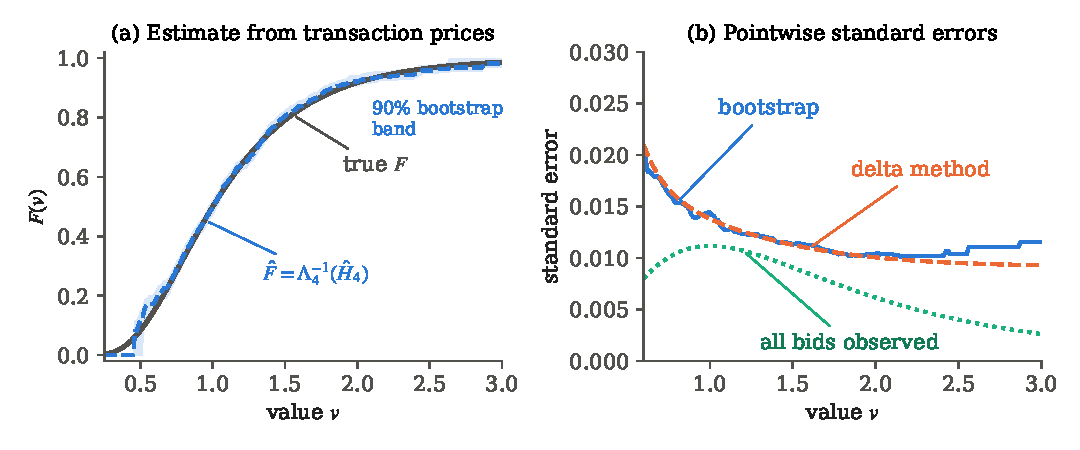
\includegraphics[width=\textwidth]{figures/ch15/asc_inversion.pdf}
\caption{Price-only inversion in simulated button auctions. Our simulation: $T=500$ auctions with $n=4$ bidders,
values lognormal with $\mu=0$ and $\sigma=\frac12$, seed 15201. Panel (a): true $F$, the estimate
$\hat F=\Lambda_4^{-1}(\hat H_4)$, and a pointwise 90 percent band from 500 bootstrap samples of whole auctions.
Panel (b): bootstrap standard error, the delta-method formula \eqref{eq:15-asc-var}, and the standard error of the
empirical CDF if all $4T$ values were observed. Panel (b) starts at $v=0.6$ because few prices fall below that
level.}\label{fig:15-asc-sim}
\end{figure}

Exogenous variation in $n$ yields one estimator $\Lambda_n^{-1}(\hat H_n)$ for each value of $n$ in the data. If
losing bids also follow the button model, each further order statistic yields another estimator through
$\Lambda_{k:n}^{-1}$. An efficient estimator would take an optimally weighted average of these estimators and impose
monotonicity of the estimated CDF \citep[Section~4.2]{AtheyHaile2007}. The differences among them are the basis of
the specification tests in \cref{thm:15-ah1}(ii).

\subsection{Asymmetric independent private values: competing risks}\label{sec:15-asym-ipv}

Independence alone suffices for identification from a single bid, provided we also observe who won. The argument
borrows from the statistics of \emph{competing risks}. A system fails as soon as one of its components fails, and
we observe the failure time and the component that failed. Up to a change of sign, this is the same as observing the
highest bid and the identity of the highest bidder \citep[footnote~21]{AtheyHaile2002}.

\begin{theorem}[{\citealp[Theorem~2]{AtheyHaile2002}}]\label{thm:15-ah2}
In the asymmetric IPV model, assume that each $F_i$ is continuous and that the support of $F_i$ is the same for all
$i$. Each $F_i$ is identified if either
\begin{enumerate}[label=(\alph*)]
\item the transaction price $B^{(n-1:n)}$ and the identity of the winner are observed, or
\item in a second-price auction, the highest bid $B^{(n:n)}$ and the identity of the winner are observed.
\end{enumerate}
Given (a) or (b), the model is testable in either of two cases.
\begin{enumerate}[label=(\roman*)]
\item Participation is exogenous, and each bidder faces at least two different sets of opponents.
\item The auction is second price, and both (a) and (b) hold.
\end{enumerate}
\end{theorem}

Independence is maintained in the theorem. What is relaxed relative to \cref{thm:15-ah1} is symmetry. We prove part
(b) for any $n$, part (a) for $n=2$, and then show the structure of part (a) for $n=3$. The general case of part (a)
is due to \citet[Theorem~1 and Section~4]{Meilijson1981}, and part (b) follows from results collected by
\citet[Theorem~7.3.1]{PrakasaRao1992}.

\begin{proof}[Proof of part (b)]
Let $\bar u$ be the upper end of the common support. For each bidder $i$ define the observable sub-distribution
\[
\tilde G_i(t)=\Pr\big(B^{(n:n)}\le t,\ I=i\big)=\int_{-\infty}^t f_i(x)\prod_{j\neq i}F_j(x)\,dx ,
\]
since bidder $i$ wins with bid $x$ when her value is $x$ and every rival's value is below $x$. The CDF of the highest
bid is $H(t)=\prod_jF_j(t)=\sum_i\tilde G_i(t)$, also observable. Differentiating $\tilde G_i$,
\[
\tilde g_i(t)=f_i(t)\prod_{j\neq i}F_j(t)=H(t)\,\frac{f_i(t)}{F_i(t)} .
\]
So the reverse hazard rate of $V_i$ equals the observable ratio $\frac{\tilde g_i(t)}{H(t)}$. Since
$\frac{f_i}{F_i}=\frac{d}{dt}\ln F_i$ and $\ln F_i(\bar u)=0$, integrating from $t$ to $\bar u$ gives
\[
F_i(t)=\exp\left(-\int_t^{\bar u}\frac{\tilde g_i(x)}{H(x)}\,dx\right).
\]
The right side is a functional of the distribution of observables.
\end{proof}

\begin{proof}[Proof of part (a) for $n=2$]
With two bidders the price is the lower value and the winner is the bidder with the higher value. For the event that
bidder 2 wins at a price of at most $t$,
\[
\tilde G_2(t)=\Pr\big(V_1\le t,\ V_1<V_2\big)=\int_{-\infty}^tf_1(x)\big(1-F_2(x)\big)\,dx .
\]
The price exceeds $t$ only if both values do, so its CDF $H$ satisfies $1-H(t)=\big(1-F_1(t)\big)\big(1-F_2(t)\big)$.
Dividing the density of $\tilde G_2$ by $1-H$ gives
\[
\frac{\tilde g_2(t)}{1-H(t)}=\frac{f_1(t)\big(1-F_2(t)\big)}{\big(1-F_1(t)\big)\big(1-F_2(t)\big)}=\frac{f_1(t)}{1-F_1(t)},
\]
the hazard rate of $V_1$. Integrating the hazard from the bottom of the support gives
$F_1(t)=1-\exp\big(-\int_{-\infty}^t\frac{\tilde g_2(x)}{1-H(x)}\,dx\big)$. The same steps with the roles reversed identify
$F_2$.
\end{proof}

With $n=3$ the argument of \citet[Section~4.1]{AtheyHaile2007} shows the structure of the general case. Let $\underline
u$ be the lower end of the support. Bidder 3 wins at a price of at most $t$ in two disjoint cases. Either both rivals
are below $t$ and bidder 3 is above $t$, or bidder 3 is below $t$ and above both rivals:
\begin{align*}
\tilde G_3(t)&=\Pr\big(V_1\le t,\ V_2\le t,\ V_3\ge t\big)+\Pr\big(V_1\le V_3,\ V_2\le V_3,\ V_3\le t\big)\\
&=F_1(t)F_2(t)\big(1-F_3(t)\big)+\int_{\underline u}^tF_1(x)F_2(x)\,dF_3(x).
\end{align*}
Integration by parts gives $\int_{\underline u}^tF_1F_2\,dF_3=F_1(t)F_2(t)F_3(t)-\int_{\underline u}^t(F_1F_2)'F_3\,dx$.
Substituting and writing $F_1(t)F_2(t)=\int_{\underline u}^t(F_1F_2)'\,dx$,
\[
\tilde G_3(t)=\int_{\underline u}^t\big(F_1(x)F_2(x)\big)'\big(1-F_3(x)\big)\,dx .
\]
Differentiating and rearranging, $(F_1F_2)'=\frac{\tilde g_3}{1-F_3}$. Integrating and taking logarithms,
\[
\ln F_1(t)+\ln F_2(t)=\ln\int_{\underline u}^t\frac{\tilde g_3(x)}{1-F_3(x)}\,dx\equiv R_3(t),
\]
and cyclically $\ln F_1+\ln F_3=R_2$ and $\ln F_2+\ln F_3=R_1$. The coefficient matrix of this system in
$(\ln F_1,\ln F_2,\ln F_3)$ has rows $(1,1,0)$, $(1,0,1)$ and $(0,1,1)$, and its determinant is $-2$. If the right
sides were known, the system would give, for example, $\ln F_1=\frac12(R_3+R_2-R_1)$. The right sides themselves
depend on the unknown distributions through $1-F_j$, so the system is a fixed-point problem.
\citet{Meilijson1981} shows that it has a unique solution.

Testability follows the logic of \cref{thm:15-ah1}. With exogenous participation, each set of opponents that bidder
$i$ faces delivers its own version of $F_i$, and the versions must agree. In a second-price auction with both (a)
and (b), the two constructions above must deliver the same $F_i$.

\casehead{Estimation}
The structure suggests a likelihood \citep[equation~(4.7)]{AtheyHaile2007}. Bidder $i$ wins at price $p$ when
some rival $j$ has value exactly $p$, every other rival $k$ has a value below $p$, and $V_i$ exceeds $p$. The
density of this event is $\big(1-F_i(p)\big)\sum_{j\neq i}f_j(p)\prod_{k\neq i,j}F_k(p)$, and the likelihood of a
sample of prices $p_t$ and winners $I_t$ is
\[
\mathcal L=\prod_{t=1}^T\big(1-F_{I_t}(p_t)\big)\sum_{j\neq I_t}f_j(p_t)\prod_{k\neq I_t,j}F_k(p_t).
\]
Parametric or semi-nonparametric maximum likelihood can be applied to it. \citet{BrendstrupPaarsch2006} develop a
semi-nonparametric estimator of this kind. Nonparametric estimators from the competing-risks literature, such as
the Kaplan-Meier estimator, are natural alternatives. \citet[Section~3.3.1]{AtheyHaile2007} make this suggestion for
the closely related problem of Dutch auctions with asymmetric bidders.

\subsection{Covariates}\label{sec:15-covariates}

Real auctions sell heterogeneous objects, and bidders differ in observable ways. Covariates are usually a nuisance,
but they can also be a source of identification.

\begin{theorem}[{\citealp[Theorem~3]{AtheyHaile2002}}]\label{thm:15-ah3}
Let private values be $V_i=g_i(A_i,Z)$, where each $g_i$ is an unknown function strictly increasing in $A_i$. Each
$F_{A_i}$ is continuous with the same support for all $i$. The auction covariates $Z$ and the transaction price are
observed, together with the identity of the winner if bidders are asymmetric.
\begin{enumerate}[label=(\roman*)]
\item If $A_1,\dots,A_n$ are independent conditional on $Z$, each conditional distribution $F_{V_i}(\cdot\mid z)$ is
identified. In the asymmetric case we assume in addition that, for each $z$, the conditional value
distributions $F_{V_i}(\cdot\mid z)$ are continuous and share a common support.
\item If $g_i(A_i,Z)=A_i+g_0(Z)$ for all $i$, and $A_1,\dots,A_n$ are mutually independent and independent of $Z$, then
the distribution of $\bm A$ and the function $g_0$ are identified up to location.
\item The symmetric models in (i) and (ii) are testable with more than one bid per auction, or with transaction
prices from auctions with exogenously varying numbers of bidders.
\end{enumerate}
\end{theorem}

\begin{proof}
(i) Fix $Z=z$. Values are independent given $z$, so \cref{thm:15-ah1} (symmetric case) or \cref{thm:15-ah2}
(asymmetric case) applies conditional on $z$. \Cref{thm:15-ah2} needs a common support of the value distributions,
which is why (i) imposes it on the $F_{V_i}(\cdot\mid z)$ directly.

(ii) Consider the symmetric case. Given $Z=z$ the price is $A^{(n-1:n)}+g_0(z)$, so its conditional CDF is
\[
H_n(b\mid z)=\Pr\big(A^{(n-1:n)}\le b-g_0(z)\big)=F_{A,(n-1:n)}\big(b-g_0(z)\big),
\]
where $F_{A,(n-1:n)}$ is the CDF of the second-highest of the $A_i$. Let $q_\tau(z)$ be the $\tau$-quantile of the
price given $z$, and $a_\tau$ the $\tau$-quantile of $A^{(n-1:n)}$. Then $q_\tau(z)=g_0(z)+a_\tau$, so
\[
g_0(z)-g_0(z')=q_\tau(z)-q_\tau(z')\quad\text{for all }z,z' ,
\]
and $g_0$ is identified up to an additive constant. A location normalization, such as $g_0(z_0)=0$ at a reference
point, fixes the constant. The price net of $g_0(Z)$ is then $A^{(n-1:n)}$, whose distribution identifies $F_A$ by
\cref{thm:15-ah1}. The asymmetric case uses \cref{thm:15-ah2} instead.

(iii) Two order statistics, or two values of $n$, give two versions of $F_{V}(\cdot\mid z)$ in (i), or of $F_A$ in
(ii), and these must coincide.
\end{proof}

\citet{AtheyHaile2002} state the support condition for the $A_i$. That suffices in (ii), where every value is
$A_i+g_0(z)$ and the supports shift together. In the asymmetric case of (i) it does not suffice, because
different functions $g_i$ need not preserve a common support. Let $A_1$ and $A_2$ be independent and uniform on
$[0,1]$, with $g_1(a)=a$ and $g_2(a)=a+2$. In an ascending auction bidder 2 always wins, at the price $A_1$.
Replacing $g_2(a)$ by $a+3$ leaves the joint distribution of the price and the winner unchanged, yet it changes
$F_{V_2}$.

Part (ii) is the basis of \emph{homogenization}. Write the price in auction $t$ as
\[
P_t=g_0(Z_t)+A_t^{(n_t-1:n_t)}=\kappa(n_t)+g_0(Z_t)+\varepsilon_t,
\qquad \kappa(n)=\E\big[A^{(n-1:n)}\big],\quad \E[\varepsilon_t\mid Z_t,n_t]=0 .
\]
A regression of prices on covariates and on indicators for $n$ estimates $g_0$, parametrically or flexibly. The
homogenized prices $P_t-\hat g_0(Z_t)$ are then treated as prices of identical objects, and the inversion of
\cref{sec:15-price-only} estimates $F_A$ \citep[equation~(6.6)]{AtheyHaile2007}. The first step matters for
inference. Suppose $\hat g_0$ converges at the parametric rate $T^{-\frac12}$. At a point $v$, the empirical CDF of
the homogenized prices then differs from its infeasible counterpart by approximately $f_{A,(n-1:n)}(v)$, the
density of $A^{(n-1:n)}$, times the average estimation error of $\hat g_0(Z_t)$. This term has the same order
$T^{-\frac12}$ as the sampling error of the empirical CDF itself.
Standard errors for $\hat F_A$ must therefore account for the first step, for example by bootstrapping both
steps together. The first step is asymptotically negligible only for second-step estimators that converge more
slowly, such as a kernel estimator of the density of $A$, under the usual smoothness conditions.
The function $g_0$ is often of interest in its own right, since it measures how observables shift valuations. In
first-price auctions the same idea requires that equilibrium bidding preserve the additive structure, which
\cref{lem:15-separability} establishes (\cref{sec:15-uh-sep} applies it to bids). Here it is immediate because
bids equal values. Alternatives to homogenization are
kernel smoothing over covariates, which \citet{HaileTamer2003} apply to ascending auctions, and flexible
mixtures for the conditional price distribution \citep[Section~6.1.1]{AtheyHaile2007}.

Bidder covariates do more. They can identify models with arbitrary correlation among values, which the next
subsection shows are not identified from bids alone. The idea comes from the Roy model, in which a worker chooses
the sector that offers the highest wage, and we observe only that wage and the chosen sector
\citep[footnote~29]{AtheyHaile2002}. Suppose $V_i=g_i(W_i)+A_i$ and suppose for a moment that the maximum value is
observed. Then
\[
\Pr\big(V^{(n:n)}\le u\mid\bm w\big)=\Pr\big(A_i\le u-g_i(w_i)\ \forall i\big)=F_{\bm A}\big(u-g_1(w_1),\dots,u-g_n(w_n)\big).
\]
The joint distribution of values is observed only along its diagonal. Variation in the indices $g_i(w_i)$, however,
moves the point at which $F_{\bm A}$ is evaluated over all of $\R^n$. When $g_j(w_j)$ is very negative for every
$j\neq i$, bidder $i$ has the highest value with probability close to one, and variation in $w_i$ traces out
$g_i$ \citep[Section~6.2.1]{AtheyHaile2007}. The following result shows that the same logic works for any single
order statistic, including the transaction price of an ascending auction.

\begin{theorem}[{\citealp[Theorem~6.1]{AtheyHaile2007}}]\label{thm:15-ah5}
Assume the following.
\begin{enumerate}[label=(\roman*)]
\item $V_i=g_i(W_i)+A_i$ for $i=1,\dots,n$.
\item $F_{\bm A}$ has support $\R^n$ and a continuously differentiable density $f_{\bm A}$.
\item The vector $(A_1,\dots,A_n)$ is independent of $(W_1,\dots,W_n)$.
\item The support of $\big(g_1(W_1),\dots,g_n(W_n)\big)$ is $\R^n$.
\item Each $g_i$ is continuously differentiable, with $g_i(w)\to\infty$ as $w\to\infty$ and $g_i(w)\to-\infty$ as
$w\to-\infty$.
\end{enumerate}
Then $F_{\bm A}$ and each $g_i$ are identified up to location from the distribution of $\big(V^{(j:n)},\bm W\big)$, for
any single $j\in\{1,\dots,n\}$.
\end{theorem}

The theorem allows arbitrary dependence among the $A_i$ and arbitrary asymmetry. It is a slight modification of
Theorem~5 of \citet{AtheyHaile2002} that corrects a minor error in its proof \citep[footnote~55]{AtheyHaile2007}. The
survey states condition (iii) pairwise, as independence of each $A_i$ and each $W_j$, while its text assumes that
the vector of the $A_i$ is independent of all covariates. The proof needs the vector form. Under pairwise
independence alone the correlation among the $A_i$ could vary with $\bm W$ while every marginal stays fixed. We
give a direct proof for scalar covariates.

\begin{proof}
Write $\bm z(u,\bm w)=\big(u-g_1(w_1),\dots,u-g_n(w_n)\big)$. For a set of bidders $\mathcal T\subseteq\{1,\dots,n\}$
define
\[
\bar F^{\mathcal T}(\bm a)=\Pr\big(A_i>a_i\ \forall i\in\mathcal T,\ A_k\le a_k\ \forall k\notin\mathcal T\big),
\]
so that $\bar F^{\emptyset}=F_{\bm A}$.

\emph{Step 1.} The $j$-th lowest value is at most $u$ exactly when at least $j$ values are at most $u$. Equivalently,
the set $\mathcal T$ of bidders with $V_i>u$ has at most $n-j$ members. Since $V_i>u$ if and only if
$A_i>u-g_i(w_i)$, and since by (iii) the distribution of $\bm A$ given $\bm W=\bm w$ is $F_{\bm A}$,
\[
\Pr\big(V^{(j:n)}\le u\mid\bm w\big)=\sum_{\mathcal T:\,|\mathcal T|\le n-j}\bar F^{\mathcal T}\big(\bm z(u,\bm w)\big).
\]

\emph{Step 2.} Write $\bar F^{\mathcal T}$ as an integral of $f_{\bm A}$ over $a_i>z_i$ for $i\in\mathcal T$ and
$a_k\le z_k$ for $k\notin\mathcal T$. Differentiating once in each $z_k$ gives a plus sign for upper limits and a
minus sign for lower limits, so
\[
\frac{\partial^n\bar F^{\mathcal T}(\bm z)}{\partial z_1\cdots\partial z_n}=(-1)^{|\mathcal T|}f_{\bm A}(\bm z).
\]

\emph{Step 3.} Since $\frac{\partial z_k}{\partial w_k}=-g_k'(w_k)$, the chain rule gives
\[
\frac{\partial^n}{\partial w_1\cdots\partial w_n}\bar F^{\mathcal T}\big(\bm z(u,\bm w)\big)
=(-1)^{|\mathcal T|}f_{\bm A}(\bm z)\prod_{k=1}^n\big(-g_k'(w_k)\big).
\]

\emph{Step 4.} Summing over the sets in Step~1, there are $\binom{n}{m}$ sets of size $m$. The identity
$\sum_{m=0}^{K}(-1)^m\binom nm=(-1)^K\binom{n-1}{K}$ follows from Pascal's rule by telescoping. With $K=n-j$ and the
case $\mathcal T=\emptyset$ of Step~3,
\[
\frac{\partial^n}{\partial w_1\cdots\partial w_n}\Pr\big(V^{(j:n)}\le u\mid\bm w\big)
=(-1)^{n-j}\binom{n-1}{n-j}\,\frac{\partial^n}{\partial w_1\cdots\partial w_n}F_{\bm A}\big(\bm z(u,\bm w)\big).
\]

\emph{Step 5.} Integrate each $\tilde w_k$ from $w_k$ to $\infty$. As $\tilde w_k\to\infty$, $g_k(\tilde w_k)\to\infty$, so
$z_k\to-\infty$ and $F_{\bm A}\to0$. Repeated use of the fundamental theorem of calculus gives
\[
\int_{w_1}^{\infty}\!\!\cdots\int_{w_n}^{\infty}\frac{\partial^nF_{\bm A}\big(\bm z(u,\tilde{\bm w})\big)}{\partial\tilde w_1\cdots\partial\tilde w_n}\,
d\tilde w_n\cdots d\tilde w_1=(-1)^nF_{\bm A}\big(\bm z(u,\bm w)\big).
\]
Combining with Step~4,
\[
F_{\bm A}\big(\bm z(u,\bm w)\big)=\frac{(-1)^j}{\binom{n-1}{n-j}}\int_{w_1}^{\infty}\!\!\cdots\int_{w_n}^{\infty}
\frac{\partial^n\Pr\big(V^{(j:n)}\le u\mid\tilde{\bm w}\big)}{\partial\tilde w_1\cdots\partial\tilde w_n}\,d\tilde w_n\cdots d\tilde w_1 ,
\]
which is equation (6.17) of \citet{AtheyHaile2007}. The right side is observable.

\emph{Step 6.} Let $w_k\to-\infty$ for every $k\neq i$. Then $z_k\to\infty$ and the left side tends to
$F_{A_i}\big(u-g_i(w_i)\big)$. This function of $(u,w_i)$ is known. Since $F_{A_i}$ is strictly increasing, any two
points with the same value satisfy $u-g_i(w_i)=u'-g_i(w_i')$, so $g_i(w_i)-g_i(w_i')=u-u'$. Hence $g_i$ is identified
up to an additive constant. With the $g_i$ known, condition (iv) lets us choose $u$ and $\bm w$ with
$\bm z(u,\bm w)$ equal to any point $\bm a\in\R^n$, which identifies $F_{\bm A}(\bm a)$.
\end{proof}

Two order statistics give two expressions for $F_{\bm A}$, and their equality is a testable restriction
\citep[Theorem~5(ii)]{AtheyHaile2002}. The result needs large support: bidder covariates must push every bidder's
value far above and far below the others'. Estimators that exploit it had not been developed when
\citet[Section~6.2.1]{AtheyHaile2007} wrote.

\subsection{Correlated values: what incomplete bids cannot reveal}\label{sec:15-nonid}

The positive results above lean on independence or on rich covariates. Without either, the picture changes.

\begin{theorem}[{\citealp[Theorem~4]{AtheyHaile2002}}]\label{thm:15-ah4}
In the symmetric private values model:
\begin{enumerate}[label=(\roman*)]
\item $F_{\bm V}$ is not identified from the vector of bids in an ascending auction.
\item In a second-price auction, $F_{\bm V}$ is not identified unless all bids are observed.
\end{enumerate}
\end{theorem}

\begin{proof}
We construct two exchangeable distributions that generate the same observables. Suppose $f_{\bm V}$ is positive on a
neighborhood of $[0,5]^n$. Let the $k$-th order statistic be the one that is not observed, where $k=n$ in an
ascending auction because the winner never exits. Fix $0<\varepsilon<\frac12$ and write $\mathcal Q(\bm c)$ for the
cube of half-width $\varepsilon$ centered at $\bm c$.

Start with $n=2$ and $k=2$, so only $\min(V_1,V_2)$ is observed. Let
\[
c(\bm v)=\indic_{\mathcal Q(1,3)}(\bm v)+\indic_{\mathcal Q(3,1)}(\bm v)-\indic_{\mathcal Q(1,2)}(\bm v)-\indic_{\mathcal Q(2,1)}(\bm v),
\]
and $\tilde f_{\bm V}=f_{\bm V}+\gamma c$ with $\gamma>0$ below the minimum of $f_{\bm V}$ on the four squares. Then
$\tilde f_{\bm V}\ge0$, and it integrates to one because the squares have equal areas. It is symmetric in $(v_1,v_2)$,
so it is exchangeable. On $\mathcal Q(1,2)$ and $\mathcal Q(1,3)$ the minimum is $v_1$, and the perturbation adds and
removes the same uniform mass for $v_1$ on $[1-\varepsilon,1+\varepsilon]$. The same holds on $\mathcal Q(2,1)$ and
$\mathcal Q(3,1)$ with the roles of the coordinates reversed. Hence the distribution of $\min(V_1,V_2)$ is unchanged.
The marginal density of $V_1$, however, gains $2\varepsilon\gamma$ on $[3-\varepsilon,3+\varepsilon]$ and loses
$2\varepsilon\gamma$ on $[2-\varepsilon,2+\varepsilon]$. Two different joint distributions, with different
marginals, generate the same observables.

For general $n$ and $k$, partition the bidders into one bidder $i$, a set of $k-1$ bidders and a set of $n-k$ bidders.
Consider the point at which the $k-1$ bidders have value 1, bidder $i$ has value 2, and the $n-k$ bidders have value
4. Shift mass $\gamma$ from the cube around this point to the cube around the point at which bidder $i$ has value 3
instead. Repeat for every such partition, which preserves exchangeability. Each shift moves only the $k$-th order statistic, from near 2
to near 3, while every other order statistic keeps the same local distribution. The joint distribution of the
observed order statistics is therefore unchanged \citep[proof of Theorem~4]{AtheyHaile2002}.
\end{proof}

\begin{figure}[htbp]
\centering
\begin{tikzpicture}[scale=0.92]
\def\e{0.3}
\fill[c15blue!7] (1-\e,5) -- (1-\e,1-\e) -- (5,1-\e) -- (5,1+\e) -- (1+\e,1+\e) -- (1+\e,5) -- cycle;
\draw[c15gray!60] (0,0) rectangle (5,5);
\draw[c15gray, densely dashed] (0,0) -- (5,5);
\draw[-{Stealth[length=2mm]}, c15gray] (0,0) -- (5.5,0) node[right] {$v_1$};
\draw[-{Stealth[length=2mm]}, c15gray] (0,0) -- (0,5.5) node[above] {$v_2$};
\foreach \x in {1,2,3,4,5} {\draw[c15gray] (\x,0) -- (\x,-0.08) node[below, font=\scriptsize] {$\x$};
  \draw[c15gray] (0,\x) -- (-0.08,\x) node[left, font=\scriptsize] {$\x$};}
\foreach \px/\py in {1/2,2/1} {\fill[c15orange!45] ({\px-\e},{\py-\e}) rectangle ({\px+\e},{\py+\e});}
\foreach \px/\py in {1/3,3/1} {\fill[c15blue!45] ({\px-\e},{\py-\e}) rectangle ({\px+\e},{\py+\e});}
\node[font=\scriptsize] at (1,2) {$-\gamma$};
\node[font=\scriptsize] at (2,1) {$-\gamma$};
\node[font=\scriptsize] at (1,3) {$+\gamma$};
\node[font=\scriptsize] at (3,1) {$+\gamma$};
\draw[-{Stealth[length=1.6mm]}, thick, c15gray] (1.42,2.25) -- (1.42,2.75);
\draw[-{Stealth[length=1.6mm]}, thick, c15gray] (2.25,1.42) -- (2.75,1.42);
\node[font=\scriptsize, align=left, anchor=west] at (2.0,4.3) {shaded strip:\\ $\min(v_1,v_2)\in[1-\varepsilon,1+\varepsilon]$};
\draw[c15gray, thin] (2.0,4.3) -- (1.25,4.0);
\end{tikzpicture}
\caption{The construction behind \cref{thm:15-ah4} for $n=2$. Mass $\gamma$ moves from the orange squares to the blue
squares, symmetrically about the diagonal. All four squares lie in the shaded strip, and within each pair the minimum
has the same distribution. The law of $\min(V_1,V_2)$, the only observable in a two-bidder ascending auction, is
therefore unchanged, while the marginal distribution of each value changes.}\label{fig:15-perturb}
\end{figure}

\Cref{fig:15-perturb} draws the construction. The intuition is a matter of dimension. Even under exchangeability,
$F_{\bm V}$ is an $n$-dimensional distribution, and identifying it from data of dimension $n-1$ or lower requires
additional restrictions \citep[Section~3.3.2]{AtheyHaile2007}. The result generalizes a classic finding of the
competing-risks literature, in which the joint distribution of risks is not identified from the distribution of the
first failure time alone \citep[footnote~26]{AtheyHaile2002}. Affiliation does not rescue identification, because a
small enough perturbation preserves strict affiliation \citep[footnote~27]{AtheyHaile2002}. The marginal $F$ itself
is not identified, so even the distribution of a single bidder's value is out of reach.

Taken together, \cref{thm:15-ah1,thm:15-ah2,thm:15-ah4,thm:15-ah5} describe a trade-off. One may relax the data,
observing only the transaction price, if values are independent. One may relax the model, allowing correlation,
if the data are richer: all bids, or bidder covariates with large support. One cannot relax both at once.
\citet{AradillasLopezGandhiQuint2013} study the case in between. With correlated private values and transaction
prices from auctions with exogenously varying numbers of bidders, $F_{\bm V}$ is not point identified. They show
that the reserve-price question does not need all of $F_{\bm V}$ \citep[pp.~88--89]{HortacsuPerrigne2021}. In an
ascending auction with reserve $r$ and seller value $v_0$, a sale occurs when $V^{(n:n)}\ge r$, at the price
$\max\{V^{(n-1:n)},r\}$. The seller's expected profit is therefore
\[
\pi(r)=\E\big[(V^{(n-1:n)}-v_0)\indic\{V^{(n-1:n)}\ge r\}\big]+(r-v_0)\Pr\big(V^{(n-1:n)}<r\le V^{(n:n)}\big),
\]
and the last probability equals $F_{(n-1:n)}(r)-F_{(n:n)}(r)$. Transaction prices identify $F_{(n-1:n)}$. Only the
distribution of the highest value at the single point $r$ is missing. It lies between $F_{(n-1:n)}(r)$ and, under
their assumptions, the value $\big[\Lambda_{n-1:n}^{-1}\big(F_{(n-1:n)}(r)\big)\big]^n$ that independence would imply.
For $r\ge v_0$ the profit falls in $F_{(n:n)}(r)$, so these limits bound $\pi(r)$. The bounds are wide.
Exogenous variation in $n$ tightens them, because the joint law of any $m<n$ values drawn at random must then
be the same in auctions of every size (p.~89, footnote 5). \Cref{sec:15-reserve-asc} reports their estimates for
timber sales.

\subsection{An incomplete model of ascending auctions}\label{sec:15-ht}

The button model is a stylized description of an English auction. In many oral auctions bidders call out prices
themselves and nontrivial minimum increments are common. A bidder may jump bid, or stay silent until the auction is
about to end \citep[Section~4.3]{AtheyHaile2007}. Bidders then fail to reveal their full willingness to
pay, and some never bid. Losing bids need not equal values, and the price need not equal the second-highest value.
\citet{HaileTamer2003} replace the button model by two weak behavioral assumptions.

\begin{assumption}[\citealp{HaileTamer2003}]\label{ass:15-ht}
Values are SIPV and the number of bidders $n$ is observed. Let $\Delta\ge0$ be the minimum bid increment.
\begin{enumerate}[label=(HT\arabic*),leftmargin=*]
\item Bidders do not bid more than they are willing to pay: $b_i\le v_i$ for every bidder.
\item Bidders do not allow an opponent to win at a price they are willing to beat: every losing bidder has
$v_i\le b^{(n:n)}+\Delta$, where $b^{(n:n)}$ is the winning bid.
\end{enumerate}
\end{assumption}

The assumptions allow the dominant-strategy behavior of the button model but do not require it. Bids need not be
monotone in values. The model is \emph{incomplete}: it restricts the relation between values and bids without fully
characterizing behavior. It cannot identify $F$, but it bounds it. Let $G_B^{(i:n)}$ be the CDF of the $i$-th lowest
bid in $n$-bidder auctions, and let $G_\Delta^{(n:n)}$ be the CDF of $B^{(n:n)}+\Delta$.

\begin{theorem}[{\citealp{HaileTamer2003} and \citealp[Theorem~4.3]{AtheyHaile2007}}]\label{thm:15-ht}
Under \cref{ass:15-ht}, $F^-(v)\le F(v)\le F^+(v)$ for all $v$, where
\[
F^+(v)=\min_{n}\ \min_{1\le i\le n}\ \Lambda_{i:n}^{-1}\big(G_B^{(i:n)}(v)\big),\qquad
F^-(v)=\max_{n}\ \Lambda_{n-1:n}^{-1}\big(G_\Delta^{(n:n)}(v)\big).
\]
\end{theorem}

\begin{proof}
\emph{Upper bound.} By HT1, $b_i\le v_i$ for every $i$. The value $v^{(i:n)}$ is at least as large as $i$ of the
values, and the bids of those $i$ bidders are no larger than their values. So at least $i$ bids are at most
$v^{(i:n)}$, which means $b^{(i:n)}\le v^{(i:n)}$. Hence the event $\{V^{(i:n)}\le v\}$ implies $\{B^{(i:n)}\le v\}$,
and
\[
G_B^{(i:n)}(v)\ge F_{(i:n)}(v)=\Lambda_{i:n}\big(F(v)\big).
\]
Applying the increasing function $\Lambda_{i:n}^{-1}$ to both sides gives $\Lambda_{i:n}^{-1}\big(G_B^{(i:n)}(v)\big)\ge F(v)$.
This holds for every $i$ and every $n$, so it holds for the minimum.

\emph{Lower bound.} By HT2, all $n-1$ losing bidders have values at most $b^{(n:n)}+\Delta$. At least $n-1$ values are
therefore below this level, so $v^{(n-1:n)}\le b^{(n:n)}+\Delta$. The event $\{B^{(n:n)}+\Delta\le v\}$ implies
$\{V^{(n-1:n)}\le v\}$, and
\[
G_\Delta^{(n:n)}(v)\le F_{(n-1:n)}(v)=\Lambda_{n-1:n}\big(F(v)\big).
\]
Applying $\Lambda_{n-1:n}^{-1}$ gives $\Lambda_{n-1:n}^{-1}\big(G_\Delta^{(n:n)}(v)\big)\le F(v)$ for every $n$, hence for the
maximum.
\end{proof}

Several features of the bounds matter in practice. If only the transaction price is recorded, the upper bound uses
$i=n$ alone. The number of bidders must be observed, which holds when bidders must register or qualify, as in the
timber auctions studied by \citet{HaileTamer2003}. If the data satisfy the button model and $\Delta\to0$, the bounds
collapse to $F$. Conversely, imposing the button model when it is false need not produce an estimate inside the
bounds, even in large samples. Imposing false structure to obtain point identification differs from selecting a
point inside the bounds of a correct incomplete model \citep[Section~4.3.1]{AtheyHaile2007}.

Estimation replaces each CDF by its empirical counterpart. Each component $\Lambda_{i:n}^{-1}(\hat G_B^{(i:n)})$ is
consistent and asymptotically normal, but the minimum and maximum have non-normal limits, and inference uses the
bootstrap. The minimum of several consistent estimators tends to select one with a downward sampling error, and the
maximum one with an upward error. The estimated bounds are therefore too narrow in finite samples and may even cross.
\citet{HaileTamer2003} replace the minimum and maximum by smooth weighted averages that approach them as the sample
grows.

\casehead{Bounds on the optimal reserve price}
The seller's main policy instrument in the SIPV model is the reserve price. Let $v_0$ be the seller's value. By
\cref{cor:14-optimal-reserve}, the optimal reserve $r^*$ solves $r^*-\frac{1-F(r^*)}{f(r^*)}=v_0$. Bounds on $F$ place
no restriction on its derivative at a point, so plugging $F^+$ or $F^-$ into this equation does not bound $r^*$. A
detour through an objective function works. Define
\[
\pi(r)=(r-v_0)\big(1-F(r)\big).
\]
Then $\pi'(r)=\big(1-F(r)\big)-(r-v_0)f(r)=-f(r)\big[\psi(r)-v_0\big]$, where $\psi$ is the virtual valuation
\eqref{eq:14-psi}. So $\pi$ has the same maximizer as the seller's expected profit, although it is not that profit when
$n>1$ \citep[footnote~34]{AtheyHaile2007}. For $r\ge v_0$, the bounds on $F$ imply
\[
\pi_1(r)\equiv(r-v_0)\big(1-F^+(r)\big)\le\pi(r)\le\pi_2(r)\equiv(r-v_0)\big(1-F^-(r)\big).
\]
Let $r_1^*$ maximize $\pi_1$, let $\pi_1^*=\pi_1(r_1^*)$, and define
\[
r^-=\sup\{r<r_1^*:\pi_2(r)\le\pi_1^*\},\qquad r^+=\inf\{r>r_1^*:\pi_2(r)\le\pi_1^*\}.
\]

\begin{proposition}[{\citealp{HaileTamer2003} and \citealp[Theorem~4.4]{AtheyHaile2007}}]\label{prop:15-ht-reserve}
Suppose $\pi$ is continuously differentiable and strictly quasi-concave. Then $r^*\in[r^-,r^+]$. Given the bounds
$F^+$ and $F^-$, the bounds $r^-$ and $r^+$ are sharp.
\end{proposition}

\begin{proof}[Proof of the inclusion]
We treat the nontrivial case $r^-<r_1^*<r^+$ and assume $\pi_2$ is continuous.
\citet[Section~4.3.2]{AtheyHaile2007} discuss the degenerate cases, in which $r^-=r^+=r_1^*$. The true objective
satisfies
$\pi(r^*)\ge\pi(r_1^*)\ge\pi_1(r_1^*)=\pi_1^*$. Suppose $r^*<r^-$. Then $r^-$ lies strictly between $r^*$ and
$r_1^*$, and strict quasi-concavity gives
\[
\pi(r^-)>\min\{\pi(r^*),\pi(r_1^*)\}\ge\pi_1^* .
\]
By continuity $\pi_2(r^-)\le\pi_1^*$, so $\pi(r^-)\le\pi_2(r^-)\le\pi_1^*$, a contradiction. The case $r^*>r^+$ is
symmetric.
\end{proof}

\Cref{fig:15-ht} applies the bounds to simulated auctions. Losing bidders stop between 80 and 100 percent of their
values, and the price may fall up to one increment below the second-highest value. The bounds contain the true
$F$ over most of the range where the data are informative. The naive estimator that treats losing bids as values
lies above the upper bound, because it ignores the fact that bidders stopped short. The implied interval for the
optimal reserve is $[0.53,1.04]$, and it contains the true optimum $0.77$ (our simulation).

\begin{figure}[htbp]
\centering
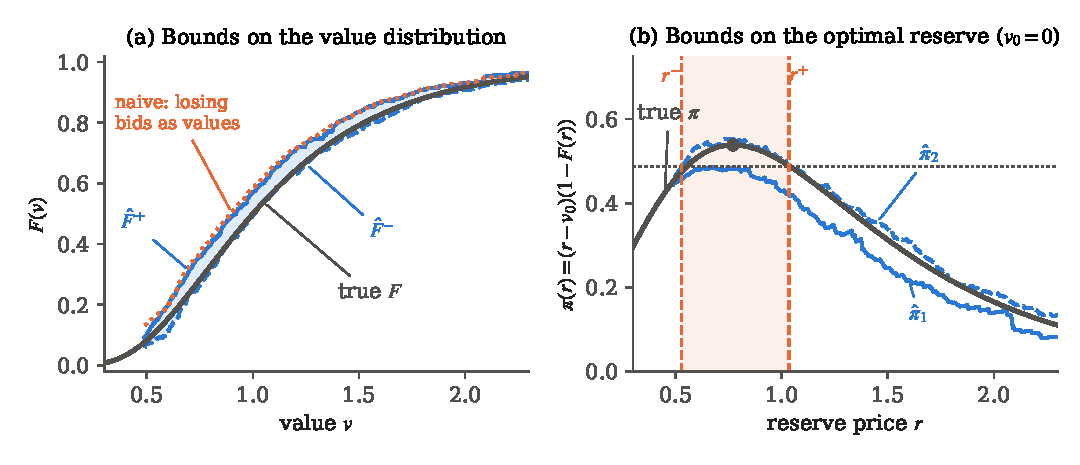
\includegraphics[width=\textwidth]{figures/ch15/ht_bounds.pdf}
\caption{Bounds from an incomplete model of ascending auctions. Our simulation: 500 auctions with $n=3$ and 500 with
$n=5$, values lognormal with $\mu=0$ and $\sigma=\frac12$, increment $\Delta=0.05$, seed 15202. Losing bidders record
bids equal to their values times a uniform draw on $[0.8,1]$. The winning bid lies between the second-highest value
minus $\Delta$ and that value, and is at least every losing bid. Panel (a): $\hat F^+$, $\hat F^-$, the true $F$ and
the naive estimate that inverts the highest losing bid as if it were the second-highest value. An order statistic is
used at $v$ only if at least 1 percent of its observations lie on each side of $v$, and curves are drawn where both
bounds are informative. Panel (b): $\hat\pi_1$, $\hat\pi_2$ and the true $\pi$ for $v_0=0$, with the interval
$[r^-,r^+]$ shaded and the true optimum marked by a dot.}\label{fig:15-ht}
\end{figure}

The approach extends in principle to asymmetric and affiliated private values, but the bounds are then likely to be
wide. Bounds on realized values reveal little about their correlation structure, and many policy questions need that
structure \citep[Section~4.3.3]{AtheyHaile2007}.

\subsection{Binding reserve prices}\label{sec:15-reserve-asc}

A reserve price $r$ inside the support of values, with $F(r)\in(0,1)$, separates potential bidders from actual
bidders. In this subsection $N$ is the number of potential bidders and $n_t$ the number who participate. With private
values a bidder participates exactly when her value is at least $r$. Under independence, the participants' values
are therefore i.i.d.\ draws from the truncated distribution
\begin{equation}\label{eq:15-truncated}
F(v\mid r)=\frac{F(v)-F(r)}{1-F(r)},\qquad v\ge r
\end{equation}
\citep[equation~(6.18)]{AtheyHaile2007}. In an ascending auction with $n_t\ge2$ participants, the price is the
second-highest of $n_t$ draws from $F(\cdot\mid r)$. With $n_t=1$ the price equals $r$.

\begin{proposition}[{\citealp[Corollary~3]{AtheyHaile2002} and \citealp[Corollary~6.1 and Theorem~6.3]{AtheyHaile2007}}]\label{prop:15-reserve-ident}
Consider the SIPV model of a first-price, second-price or ascending auction with reserve price $r$ and
$F(r)\in(0,1)$.
\begin{enumerate}[label=(\roman*)]
\item Consider a second-price or ascending auction, or a first-price auction whose participants learn their number
before they bid. If one bid from each auction and the number of participants are observed, $F(\cdot\mid r)$ is
identified on $[r,\infty)$.
\item The model is testable if two bids from each auction are observed, or if one bid is observed in auctions with
different numbers of participants.
\item If $N$ is fixed and the number of participants is observed, $N$ and $F(r)$ are identified. Combined with (i),
$F(v)$ is then identified for every $v\ge r$.
\item Consider a first-price auction whose bidders know $N$ but not the number of participants when they bid. If $N$
is fixed and one bid from each auction and the number of participants are observed, then $N$, $F(r)$ and $F(v)$
for every $v\ge r$ are identified.
\end{enumerate}
\end{proposition}

\begin{proof}
Parts (i) and (ii) apply \cref{thm:15-ah1} to the truncated distribution \eqref{eq:15-truncated}, conditioning on
the number of participants. In second-price and ascending auctions this is valid because bidding one's value is
a dominant strategy. In a first-price auction whose participants know their number $n_t$, each participant faces
$n_t-1$ rivals with values drawn from $F(\cdot\mid r)$, and the inversion of \cref{sec:15-gpv} applies to that
distribution. In the setting of (iv), condition (C2) of \cref{thm:15-gpv-reserve} makes participants' bids
i.i.d.\ given their number, with a distribution that does not depend on that number. Two bids per auction, or one
bid at different numbers of participants, then give two versions of that distribution, and these must coincide.
For part (iii), each potential bidder participates independently with probability $1-F(r)$, so the
number of participants is binomial with parameters $N$ and $1-F(r)$. Its distribution determines both parameters. Exchangeability gives a
convenient formula. The probability that a given bidder stays out is the same for every bidder. It therefore
equals the expected fraction of bidders who stay out:
\[
F(r)=\Pr(\text{bidder 1 does not bid})=\frac{\E[N-n_t]}{N}=\sum_{k=1}^{N}\frac{k}{N}\Pr\big(n_t=N-k\big),
\]
which is equation (6.19) of \citet{AtheyHaile2007}. Finally, \eqref{eq:15-truncated} gives
$F(v)=F(r)+\big(1-F(r)\big)F(v\mid r)$ for $v\ge r$.

For part (iv), a participant who bids $b\ge r$ wins when each of her $N-1$ potential rivals either stays out or bids
less. Her win probability therefore depends on $N$ and $F(r)$, and the inversion conditional on $n_t$ misstates her
first-order condition. Take $N=2$, values uniform on $[0,1]$ and $r=\frac12$, for example. The equilibrium bid is
$\beta(v)=\frac{v}{2}+\frac{1}{8v}$. Applied to two-participant auctions, the inversion of \cref{sec:15-gpv} maps
the bid of a bidder with value $\frac34$ to about $0.611$. The correct inversion \eqref{eq:15-gpv-reserve} uses
$N$ and $F(r)$, which part (iii) identifies. Given their number, participants' bids are i.i.d., so the observed
bid and that number identify the distribution of a participant's bid. When the observed bid is the highest, this
step is the root formula of \cref{prop:15-winbid}. \Cref{thm:15-gpv-reserve} then gives $F(v)$ for $v\ge r$.
\end{proof}

\citet[Corollary~3]{AtheyHaile2002} state (i) for first-price auctions as well, without saying what bidders know
about participation. The information structure matters. Part (iv) adopts that of \citet{GuerrePerrigneVuong2000},
in which bidders do not see who participates, and \cref{sec:15-gpv-reserve} develops it.

The sample analog of the formula that completes part (iii), $\hat F(v)=\hat F(r)+\big(1-\hat F(r)\big)\hat F(v\mid r)$, is consistent. Below
the reserve the data are silent without parametric assumptions. Is the truncated distribution enough for the
reserve-price question? The next result says that it usually is.

\begin{proposition}[{\citealp[Theorem~6.2]{AtheyHaile2007}}]\label{prop:15-trunc-reserve}
For a univariate CDF $\Phi$, let $\pi(\tilde r;\Phi)=(\tilde r-v_0)\big(1-\Phi(\tilde r)\big)$ and let $p^*(\Phi)$ maximize
$\pi(\cdot;\Phi)$ over the support of $\Phi$. Suppose $\pi(\cdot;F)$ is continuously differentiable and strictly
quasi-concave, and write $F_{\mid r}=F(\cdot\mid r)$.
\begin{enumerate}[label=(\roman*)]
\item If $r<p^*(F)$, then $p^*(F_{\mid r})=p^*(F)$.
\item If $r\ge p^*(F)$, then $p^*(F_{\mid r})=r$.
\end{enumerate}
\end{proposition}

\begin{proof}
For $\tilde r\ge r$, \eqref{eq:15-truncated} gives $1-F(\tilde r\mid r)=\frac{1-F(\tilde r)}{1-F(r)}$, so
\[
\pi(\tilde r;F_{\mid r})=\frac{\pi(\tilde r;F)}{1-F(r)}\qquad\text{for all }\tilde r\ge r .
\]
On the support of $F_{\mid r}$ the two objectives differ by a positive multiplicative constant. If $r<p^*(F)$, the
unconstrained maximizer lies in $[r,\infty)$ and both objectives peak there. If $r\ge p^*(F)$, strict
quasi-concavity makes $\pi(\cdot;F)$ decreasing on $[r,\infty)$, so the truncated objective peaks at its lower end
$r$.
\end{proof}

In the SIPV model, the optimal reserve computed from participants alone, ignoring the selection created by the
reserve, is the true optimum unless the actual reserve already exceeds it. The data reveal when that happens,
because the estimated optimum then sits at the actual reserve. Variation in reserve prices across auctions does more.
Suppose reserves vary for reasons unrelated to values. Data from auctions with low reserves then reveal $F$ over a
longer range, and a reserve below the lower end of the support reveals all of $F$
\citep[Section~6.3.1]{AtheyHaile2007}. Reserve prices may instead respond to features of the object that bidders see
and the econometrician does not. A reserve then signals unobserved quality, and treating it as an exogenous
truncation point is a mistake. \citet{Roberts2013} builds an identification
strategy on this observation (\cref{sec:15-uh}). With a reserve price, the tests of private against common values
in \cref{sec:15-cv} remain available, because truncation at a common reserve preserves exchangeability
\citep[Corollary~4]{AtheyHaile2002}.

\casehead{Applications to timber sales}
Timber sales have been the main testing ground for these methods \citep[Section~2.1]{HortacsuPerrigne2021}.
The estimates agree on one point. Observed reserve prices are low relative to the optimum that most
models imply, and the gain from raising them depends on the information structure.

\citet{Paarsch1997} studies ascending timber auctions in British Columbia with a parametric model (pp.~87--88).
He treats the winning bid as the second-highest value, as in the button model. Bids are per species on
estimated volumes, while payments follow harvested volumes. He therefore rewrites each value in terms of an
average harvesting cost, and the winner is the bidder with the lowest cost. He specifies a parametric cost
function and a Weibull distribution. The estimated optimal reserve is then on average 3.4 to 4.2 times the
observed reserve, as the seller's value $v_0$ ranges from zero to the appraisal value of the timber.

\citet{HaileTamer2003} apply \cref{thm:15-ht,prop:15-ht-reserve} to Forest Service ascending auctions, with
data from Oregon (p.~88). They estimate bounds on the optimal reserve and on the implied gain. The increase in
the seller's profit ranges from little to 34 percent, depending on $v_0$. At high values of $v_0$ the optimal
reserve leaves more than 90 percent of tracts unsold. \citet{AradillasLopezGandhiQuint2013} use Oregon data
as well (p.~89). Their estimated bounds on the seller's profit are smaller than the profit computed under
independent values, and independence also overstates bidders' surplus. A reserve computed under independence
would be too high and could even lower the seller's profit. The authors note that an optimal reserve would
conflict with the Forest Service's mandate to sell about 85 percent of the tracts it offers. The mandate may
explain why observed reserves are low.

\citet{CoeyEtAl2017} exploit the asymmetry between loggers and mills of \cref{sec:15-als} to tighten
the bounds in California sales (p.~89). The lower bound on the optimal reserve is similar, while the upper bound
is 10 to 15 percent lower. \citet{CoeyLarsenSweeney2019} turn to the \emph{bidder exclusion effect}, the expected
fall in revenue when one of $N$ bidders is excluded at random (pp.~89--90). In an ascending auction with
private values the price is the second-highest value. Excluding a bidder lowers it to the third-highest value
exactly when the excluded bidder holds one of the two highest values, which happens with probability
$\frac{2}{N}$. The exclusion effect is therefore
\[
\frac{2}{N}\,\E\big[B^{(N-1:N)}-B^{(N-2:N)}\big],
\]
which needs two order statistics and the number of potential bidders. Under exogenous participation the
observed fall in revenue, $\E[B^{(N-1:N)}]-\E[B^{(N-2:N-1)}]$, must equal this effect. The difference is their
test statistic. A negative value is consistent with common values, and a zero value with private values, as
\citet{AtheyHaile2002} show \citep[footnote~6]{HortacsuPerrigne2021}. The same effect bounds the gain from an
optimal reserve without computing the reserve. By \cref{prop:14-bk}, an optimal reserve with $N-1$ bidders
raises less revenue than one more bidder without a reserve. In California sales the average revenue gain from
an optimal reserve is at most 13 percent. Exogenous participation is rejected, with positive selection, since
values tend to be higher in auctions with more participants (p.~90).

The first-price evidence points the same way. \citet{LiPerrigne2003} study French public timber sales by
first-price sealed bid with a secret reserve (p.~90). They model the reserve as random, equal to the seller's
value and independent of bidders' values, which are independent private values. The inversion of
\citet{GuerrePerrigneVuong2000}, developed in \cref{sec:15-gpv}, recovers the value distribution. The optimal announced reserve is on average 46 percent higher
than the secret one. It lowers the number of successful sales and raises total revenue only slightly, but it
doubles the seller's net profit.

\section{First-Price Auctions I: The Inversion Problem and Direct Methods}\label{sec:15-direct}

In first-price and Dutch auctions bidders shade their bids below their values, and the amount of shading depends on
the distribution of values. This section explains why that makes identification and estimation harder. It then
studies the direct route, maximum likelihood with its non-regularity and the simulated estimator of
\citet{LaffontOssardVuong1995}. It closes with a comparison of direct and indirect methods that motivates
\cref{sec:15-gpv}.

\subsection{Why first-price auctions are harder}\label{sec:15-fpa-hard}

In the SIPV model with reserve price $r$, a bidder with value $v\ge r$ bids (\cref{prop:14-rs})
\[
\beta(v)=v-\frac{\int_r^vF(t)^{n-1}\,dt}{F(v)^{n-1}} .
\]
Bids are observed and values are not. The bid function depends on the unknown $F$, the very object we want to
estimate \citep[Section~3.1]{AtheyHaile2007}. The distribution of bids $G(b)=F\big(\beta^{-1}(b)\big)$ therefore depends
on $F$ in two ways, directly through the distribution of values and indirectly through the equilibrium strategy
\citep[p.~529]{GuerrePerrigneVuong2000}. Even a closed-form bid function does not tell us how to recover $F$ from $G$.

The economics of shading also suggests the way out. A bidder trades off the probability of winning against the
surplus she earns when she wins. In a procurement auction a firm with cost $c$ chooses its bid $b$ to maximize
$(b-c)\Pr(\text{win}\mid b)$, exactly as an oligopolist chooses its price to maximize $(p-c)q(p)$. The win probability
plays the role of residual demand, and the first-order condition is an inverse elasticity rule
(see \eqref{eq:14-proc-foc} and \eqref{eq:14-proc-lerner}, and \cref{ch:theory}). In demand estimation we recover marginal costs from the
pricing first-order condition once demand is estimated (\cref{ch:diffprod,ch:blp}). In auctions we can recover values
from the bidding first-order condition once the distribution of rivals' bids is estimated. That is the indirect route
of \cref{sec:15-gpv}. The literature first took the direct route, which we study now.

\subsection{Maximum likelihood and its non-regularity*}\label{sec:15-ml}

Let $F(\cdot;\theta)$ be a parametric family with density $f(\cdot;\theta)$, $\theta\in\Theta\subset\R^K$, and suppose
for simplicity that there is no binding reserve price. Each bid is $B_{it}=\beta(V_{it};\theta)$ with $\beta$ strictly
increasing, so $G(b;\theta)=F\big(\beta^{-1}(b;\theta);\theta\big)$. Differentiating gives the bid density
\begin{equation}\label{eq:15-bid-density}
g(b;\theta)=\frac{f\big(\beta^{-1}(b;\theta);\theta\big)}{\beta'\big(\beta^{-1}(b;\theta);\theta\big)},
\qquad b\in\big[\beta(\underline v;\theta),\ \beta(\bar v(\theta);\theta)\big].
\end{equation}
The equilibrium differential equation \eqref{eq:14-rs-ode} gives $\beta'(v)=(n-1)\big(v-\beta(v)\big)\frac{f(v)}{F(v)}$.
Substituting it, with $\xi=\beta^{-1}(b;\theta)$,
\[
g(b;\theta)=\frac{F(\xi;\theta)}{(n-1)(\xi-b)} .
\]
The log-likelihood of all bids is $\ell(\theta)=\sum_t\sum_i\ln g(b_{it};\theta)$. If only the winning bid is
recorded, as in a Dutch auction, its CDF is $H(b;\theta)=F(\xi;\theta)^n$. Its density is
\[
h(b;\theta)=\frac{nF(\xi;\theta)^{n-1}f(\xi;\theta)}{\beta'(\xi;\theta)}=\frac{n}{n-1}\,\frac{F(\xi;\theta)^n}{\xi-b},
\]
which is equation (7) of \citet{LaffontOssardVuong1995}. With a binding reserve price the object goes unsold with
probability $F(r;\theta)^n$, and the likelihood takes a Tobit form with a mass point at $r$.

Maximum likelihood faces three obstacles. The first is computation. Each evaluation of $\ell(\theta)$ requires
$\beta^{-1}(b_{it};\theta)$ for every bid and every trial value of $\theta$. The bid function involves an integral and
has no closed form for most families. With asymmetric or affiliated values it solves a system of differential
equations, such as \eqref{eq:14-asym-foc}, which must be solved anew at each $\theta$. The second obstacle is regularity. The
upper end of the support of bids, $\beta(\bar v(\theta);\theta)$, depends on $\theta$. With only the winning bid, the
support is $[r,\E\max(Y,r)]$, where $Y$ is the largest of $n-1$ draws from $F$ \citep[p.~958]{LaffontOssardVuong1995}.
A parameter-dependent support violates the standard conditions for maximum likelihood (\cref{sec:A-mle-nonregular}).
The third obstacle is that practical applications were confined to families with closed-form bid functions and to
the SIPV model \citep[Section~3.2]{AtheyHaile2007}. \citet{DonaldPaarsch1993,DonaldPaarsch1996} study the
non-regular problem. They derive non-standard asymptotic distributions and propose estimators built on extreme order
statistics of the bids. The following example shows what goes wrong.

\begin{example}[Maximum likelihood with power-distributed values]\label{ex:15-power-mle}
Let $F(v;\theta)=\big(\frac{v}{\theta}\big)^\gamma$ on $[0,\theta]$ with $\gamma>0$ known and $\theta$ unknown, and let
there be no reserve price. As in \cref{ex:14-power}, rescaled to the support $[0,\theta]$,
\[
\int_0^v\Big(\frac{t}{\theta}\Big)^{\gamma(n-1)}dt=\frac{v}{\gamma(n-1)+1}\Big(\frac{v}{\theta}\Big)^{\gamma(n-1)}.
\]
Substituting into \eqref{eq:14-rs-bid} gives
\[
\beta(v)=v-\frac{v}{\gamma(n-1)+1}=c\,v,\qquad c=\frac{\gamma(n-1)}{\gamma(n-1)+1}.
\]
Bids $B=cV$ have CDF $G(b;\theta)=\big(\frac{b}{c\theta}\big)^\gamma$ on $[0,c\theta]$ and density
$g(b;\theta)=\gamma b^{\gamma-1}(c\theta)^{-\gamma}$. With $nT$ bids the likelihood is
\[
L(\theta)=\prod_{t=1}^T\prod_{i=1}^n\gamma\,b_{it}^{\gamma-1}(c\theta)^{-\gamma}\,\indic\big(b_{it}\le c\theta\big)
=\Big[\prod_{t,i}\gamma\,b_{it}^{\gamma-1}\Big](c\theta)^{-\gamma nT}\,\indic\Big(\theta\ge\frac{\max_{t,i}b_{it}}{c}\Big).
\]
The likelihood is zero for $\theta$ below $\frac{1}{c}\max_{t,i}b_{it}$ and strictly decreasing above it, so
\[
\hat\theta=\frac{1}{c}\max_{t,i}b_{it}.
\]
Its distribution follows from that of the maximum of $nT$ independent bids. For $0\le x\le T\theta$,
\[
\Pr\big(T(\theta-\hat\theta)>x\big)=\Pr\Big(\max_{t,i}B_{it}<c\Big(\theta-\frac{x}{T}\Big)\Big)
=\Big(1-\frac{x}{T\theta}\Big)^{\gamma nT}\longrightarrow e^{-\frac{\gamma n}{\theta}x}.
\]
So $T(\theta-\hat\theta)$ converges to an exponential distribution with mean $\frac{\theta}{\gamma n}$.
\end{example}

The estimator converges at rate $T$, faster than the usual $\sqrt T$, and its limit is not normal. The information
equality fails. The score of one bid is $\frac{\partial}{\partial\theta}\ln g(b;\theta)=-\frac{\gamma}{\theta}$, whose mean is not
zero, because the support moves with $\theta$. Standard errors from the inverse information matrix are therefore
invalid, and the nonparametric bootstrap fails for the sample maximum (\cref{prop:A-uniform-mle} and
\cref{sec:A-boot-fail}). The estimator also rests entirely on the largest bid, so a single error in the top bid moves
it. The same structure arises whenever the upper end of the bid support depends on the parameters, which is the rule
in first-price auctions.

\subsection{Laffont, Ossard and Vuong (1995): simulated nonlinear least squares*}\label{sec:15-lov}

\casehead{Question}
\citet{LaffontOssardVuong1995} ask how to estimate a general parametric distribution of private values from
first-price or Dutch auctions in which only the winning bid is observed. They want to allow heterogeneity across
auctions and an unknown number of bidders, and to avoid computing the equilibrium bid function. Earlier structural
work by \citet{Paarsch1992} had relied on families with closed-form bid functions
\citep[p.~954]{LaffontOssardVuong1995}.

\casehead{Model}
The model of their Section~2 is the SIPV first-price auction with reserve price $r_t$ and $n$ bidders. The
equilibrium bid (their eq.~(1)) is \eqref{eq:14-rs-bid}. The winning bid is $\beta\big(V_t^{(n:n)}\big)$ when
$V_t^{(n:n)}\ge r_t$ (eq.~(2)), and the optimal reserve solves $r^*=v_0+\frac{1-F(r^*)}{f(r^*)}$ (eq.~(4),
\cref{cor:14-optimal-reserve}). Heterogeneity enters through observed characteristics $z_t$:
\[
F_t(\cdot)=F(\cdot\mid z_t,\theta)\qquad\text{(their eq.~(5))}.
\]
The reserve price is not among the characteristics, which fits their application, where buyers and sellers have the
same information about market conditions \citep[p.~957]{LaffontOssardVuong1995}. To avoid a discontinuity when the
object is unsold, they set the winning bid equal to the reserve in that case (eq.~(6)):
\[
b^w_t=\beta_t\big(V_t^{(n:n)}\big)\,\indic\big(V_t^{(n:n)}\ge r_t\big)+r_t\,\indic\big(V_t^{(n:n)}<r_t\big).
\]
Its distribution has a mass $F_t(r_t)^n$ at $r_t$ and the density $h_t$ above $r_t$. Bidders draw new independent values
in every auction, which rules out the dynamic incentives of repeated auctions.

\casehead{Revenue equivalence as an estimation device}
The key step replaces the intractable bid function by a conditional expectation that is easy to simulate.

\begin{lemma}[\citealp{LaffontOssardVuong1995}, eq.~(12)]\label{lem:15-lov}
For $v\ge r$, $\ \beta(v)=\E\big[\max\{V^{(n-1:n)},r\}\mid V^{(n:n)}=v\big]$.
\end{lemma}

\begin{proof}
Given that the highest of $n$ i.i.d.\ values equals $v$, the other $n-1$ values are i.i.d.\ draws from $F$ truncated
to lie below $v$. Their maximum $V^{(n-1:n)}$ then has CDF $\big(\frac{F(y)}{F(v)}\big)^{n-1}$ on $y\le v$. This is the
distribution of the highest rival value $Y_1$ conditional on $Y_1<v$. Hence the right side equals
$\E\big[\max\{Y_1,r\}\mid Y_1<v\big]$, which is $\beta(v)$ by \eqref{eq:14-rs-condexp}.
\end{proof}

Applying the lemma at $v=V_t^{(n:n)}$ gives $b^w_t=\E\big[\max\{V_t^{(n-1:n)},r_t\}\mid V_t^{(n:n)}\big]$. The equality
also holds when the object is unsold, since both sides then equal $r_t$. Taking expectations conditional on
$x_t=(r_t,z_t)$ yields the moment that drives the estimator (their eqs.~(13)--(15)):
\begin{equation}\label{eq:15-lov-mean}
\begin{aligned}
m_t(\theta)\equiv\E\big[b^w_t\mid x_t\big]&=\E\big[\max\{V_t^{(n-1:n)},r_t\}\mid x_t\big]\\
&=\int\!\!\cdots\!\int\max\{u^{(n-1:n)},r_t\}\prod_{i=1}^nf_t(u_i)\,du_1\cdots du_n ,
\end{aligned}
\end{equation}
where $u^{(n-1:n)}$ is the second highest of $(u_1,\dots,u_n)$. This is revenue equivalence (\cref{prop:14-ret}). The
expected winning bid in a first-price auction equals the expected price in an English auction with the same reserve.
The right side needs no bid function: draw $n$ values, take the second highest, and compare it with the reserve.

\casehead{The simulator}
\citet{LaffontOssardVuong1995} use importance sampling. For each auction they choose a known density $g_t$ whose
support contains that of $f_t$. Before estimation they draw $S$ independent samples
$\bm u_t^s=(u^s_{1t},\dots,u^s_{nt})$, $s=1,\dots,S$, with each $u^s_{it}$ drawn from $g_t$. Their eqs.~(16)--(17) define
\[
X_{st}(\theta)=\max\big\{u^{s}_{(n-1:n)t},\,r_t\big\}\prod_{i=1}^n\frac{f_t(u^s_{it};\theta)}{g_t(u^s_{it})},
\qquad\bar X_t(\theta)=\frac1S\sum_{s=1}^SX_{st}(\theta).
\]
By construction $\E\big[\bar X_t(\theta)\mid x_t\big]=m_t(\theta)$. The draws do not depend on $\theta$ and are independent of
$b^w_t$ given $x_t$. Because $\theta$ enters only through the weights, outside the maximum, $\bar X_t(\theta)$ is twice
continuously differentiable in $\theta$ whenever $f$ is. Standard derivative-based optimization then applies, and the
asymptotic theory is simpler than for discontinuous simulators \citep[p.~961]{LaffontOssardVuong1995}.

\casehead{The bias of naive simulated least squares}
Nonlinear least squares with the exact mean would minimize $\frac1T\sum_t\big(b^w_t-m_t(\theta)\big)^2$. Replacing
$m_t$ by its simulator gives the naive criterion $Q_S(\theta)=\frac1T\sum_t\big(b^w_t-\bar X_t(\theta)\big)^2$ (their
eq.~(8)). To find its limit, decompose
\[
b^w_t-\bar X_t(\theta)=\big(b^w_t-m_t(\theta_0)\big)+\big(m_t(\theta_0)-m_t(\theta)\big)+\big(m_t(\theta)-\bar X_t(\theta)\big).
\]
Given $x_t$, the first and third terms have mean zero and are independent of each other, and the second is fixed.
Every cross product therefore has conditional mean zero, and
\[
\E\Big[\big(b^w_t-\bar X_t(\theta)\big)^2\,\Big|\,x_t\Big]=\sigma_0^2(x_t)+\big(m_t(\theta_0)-m_t(\theta)\big)^2+\frac1S\,\omega_t(\theta),
\]
where $\sigma_0^2(x_t)=\Var(b^w_t\mid x_t)$ and $\omega_t(\theta)=\Var\big(X_{st}(\theta)\mid x_t\big)$. The first term does not
depend on $\theta$ and the second is minimized at $\theta_0$. The third term, the simulation variance, does depend on
$\theta$. The naive estimator converges to the minimizer of the sum of the last two terms, which is generally not
$\theta_0$ (their eq.~(9)). It favors parameter values at which the simulator is less noisy, and it is inconsistent for
any fixed $S$.

The fix subtracts an unbiased estimate of the simulation variance. The sample variance of the draws, divided by
$S$, satisfies $\E\big[\frac{1}{S(S-1)}\sum_s\big(X_{st}(\theta)-\bar X_t(\theta)\big)^2\mid x_t\big]=\frac1S\omega_t(\theta)$. The
simulated nonlinear least squares (SNLS) criterion is therefore (their eq.~(11))
\begin{equation}\label{eq:15-snls}
Q_S^*(\theta)=\frac1T\sum_{t=1}^T\left[\big(b^w_t-\bar X_t(\theta)\big)^2-\frac{1}{S(S-1)}\sum_{s=1}^S\big(X_{st}(\theta)-\bar X_t(\theta)\big)^2\right].
\end{equation}
Each bracket has conditional mean $\sigma_0^2(x_t)+\big(m_t(\theta_0)-m_t(\theta)\big)^2$, the same as the criterion of exact
nonlinear least squares. \Cref{sec:A-snlls} treats the estimator in the general framework of simulation estimators.

\casehead{Asymptotic properties}
Their Proposition~1 shows that for any fixed $S$ the SNLS estimator $\hat\theta$ is strongly consistent as $T\to\infty$,
provided $\theta_0$ is identified from the first moment of the winning bid. The minimized criterion $Q_S^*(\hat\theta)$
consistently estimates the mean squared error of the model. Proposition~2 gives asymptotic normality. Let
$\mu_t=\frac{\partial m_t(\theta_0)}{\partial\theta}$ and $Y_{st}=\frac{\partial X_{st}(\theta_0)}{\partial\theta}$, and let $\omega_t$,
$\Omega_t$ and $C_t$ be the conditional variances of $X_{st}(\theta_0)$ and $Y_{st}$ and their conditional covariance. Then
$\Sigma^{-\frac12}\sqrt T(\hat\theta-\theta_0)\xrightarrow{d}N(0,I_K)$ with $\Sigma=A^{-1}BA^{-1}$ and
\begin{align*}
A&=\frac1T\sum_{t=1}^T\E\big[\mu_t\mu_t^\top\big],\\
B&=\frac1T\sum_{t=1}^T\E\left[\sigma_0^2(x_t)\mu_t\mu_t^\top+\frac1S\Big(\sigma_0^2(x_t)\Omega_t+\omega_t\mu_t\mu_t^\top\Big)
+\frac{1}{S(S-1)}\Big(\omega_t\Omega_t+C_tC_t^\top\Big)\right].
\end{align*}
The first term of $B$ alone gives the sandwich of exact nonlinear least squares. Simulation inflates the variance by a
term of order $\frac1S$, which vanishes as $S$ grows. Proposition~3 gives a heteroskedasticity-robust estimator of
$\Sigma$ that is consistent for fixed $S$ and requires neither $\sigma_0^2$ nor exact moments. Competing simulated
estimators, such as simulated maximum likelihood, are inconsistent for fixed $S$, because they simulate a nonlinear
function of an expectation \citep[p.~962]{LaffontOssardVuong1995}.

\casehead{An unknown number of bidders}
Bidders in a Dutch auction who never bid leave no trace, so $n$ may be unknown. Their Proposition~4 treats the true
$n_0$ as a parameter in a bounded set $\mathcal J$ of integers. For each $n\in\mathcal J$ compute $\hat\theta_n$ and
$Q^*_{S,n}(\hat\theta_n)$, and let $\hat n$ minimize the criterion over $\mathcal J$. Then $(\hat n,\hat\theta_{\hat n})$ converges almost
surely to $(n_0,\theta_0)$ for fixed $S$. Since $\hat n$ is discrete it converges faster than $\hat\theta$, and inference on
$\theta$ can proceed as if $n$ were known (their footnote~14). Identification of $n$ here rests on the parametric
family. Without $n$, the distribution of the winning bid does not even determine the distribution of a single bid
\citep[Section~3.3.1]{AtheyHaile2007}, as \cref{sec:15-gpv-winbid} shows.

\casehead{Extensions}
Three extensions broaden the method. First, if the econometrician observes only part $z_{1t}$ of the
characteristics $z_t=(z_{1t},z_{2t})$ that bidders see, a parametric model $h(z_2\mid r,z_1;\gamma)$ for the omitted part
can be integrated out. The simulator then draws $z_{2t}$ along with the values (their eqs.~(24)--(25)). Second, the
lemma lets us simulate $\beta(v)$ itself, by averaging $\max\{V^{(n-1:n)},r\}$ over draws given $V^{(n:n)}=v$. Higher
moments of the winning bid then become available for a method of simulated moments. Third, the moment
\eqref{eq:15-lov-mean} is the expected price of any standard auction with the same reserve, so the estimator applies
equally to English and second-price auctions \citep[p.~959]{LaffontOssardVuong1995}.

\casehead{Setting and data}
The application is a descending auction of greenhouse eggplants in Marmande, France. The sellers are farmers, and
the buyers are resale trading firms acting for retailers who placed orders at given prices before the market
opened. These prices are the buyers' valuations, which supports the private values assumption. In each round a
case of 15 to 350 kilos is offered. The seller announces a reserve price per kilo, and the clock starts high, for
example at fifteen francs when the usual price is about ten francs per kilo. The first buyer to stop the clock wins
and pays the current price \citep[p.~967]{LaffontOssardVuong1995}.

The data cover daily sales in the summer of 1990, from June to October. To avoid dynamic incentives within a day,
the authors keep only days on which a single case of a given size category was offered. Eggplants deteriorate
quickly, so one day's supply can be treated as independent of the previous day's trade. The sample has 81 auctions.
The winning bid averages 7.52 francs per kilo (standard deviation 2.21, range 2.00 to 11.98), and the reserve price
averages 6.43 (standard deviation 1.81, range 2.00 to 10.00). The correlation between winning bids and reserves is
0.962 \citep[Appendix~B]{LaffontOssardVuong1995}.

\begin{figure}[htbp]
\centering
\begin{subfigure}[t]{0.49\textwidth}
\centering
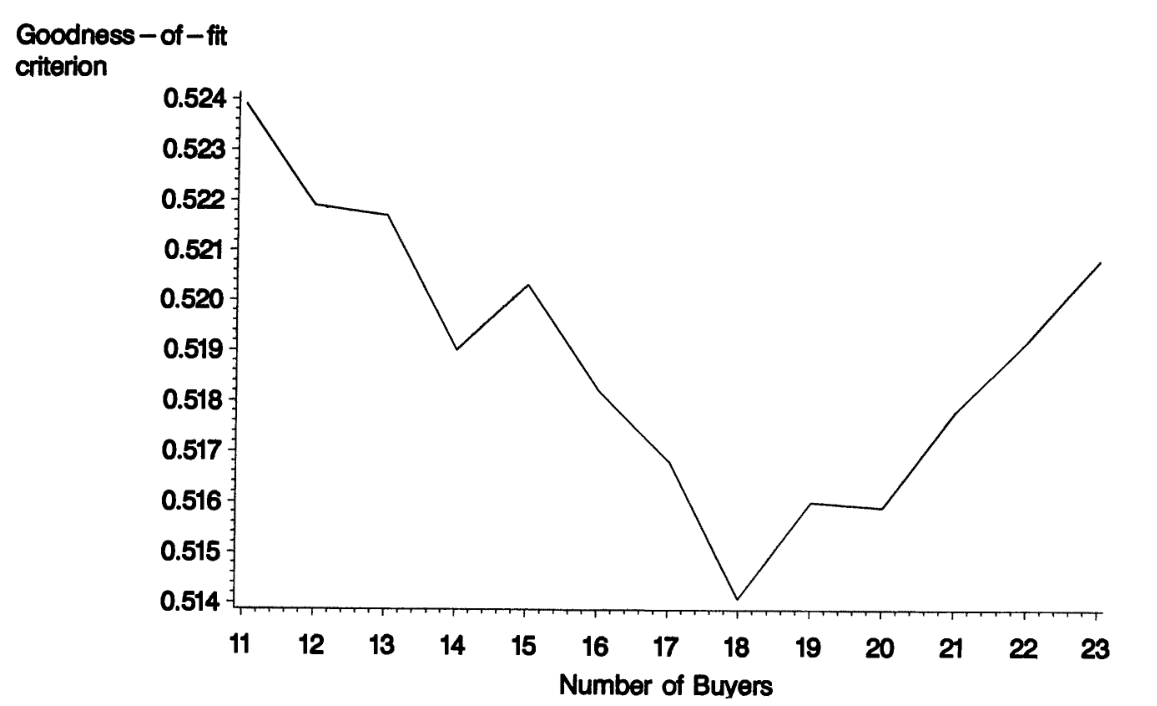
\includegraphics[width=\textwidth]{figures/ch15/lov1995_fig1.png}
\caption{Criterion $Q_S^*(\hat\theta_n)$ against the assumed number of buyers $n$.}\label{fig:15-lov-n}
\end{subfigure}\hfill
\begin{subfigure}[t]{0.49\textwidth}
\centering
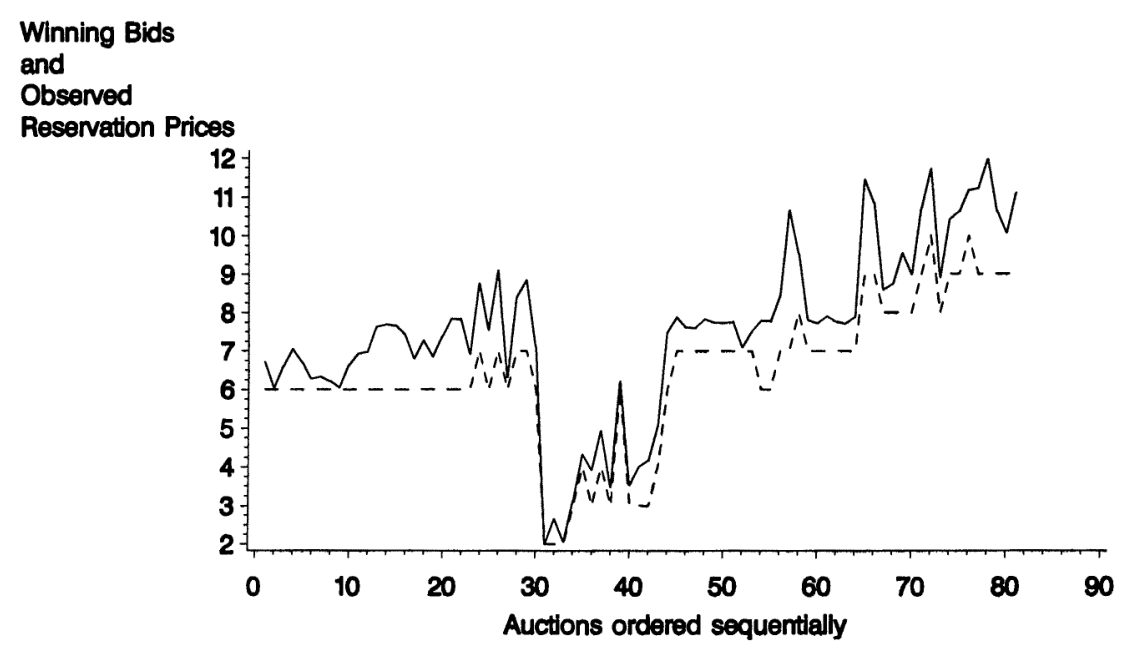
\includegraphics[width=\textwidth]{figures/ch15/lov1995_fig3.png}
\caption{Winning bids (solid) and reserve prices (dashed), auctions in chronological order.}\label{fig:15-lov-reserve}
\end{subfigure}
\caption{The Marmande eggplant auctions. Panel (a) selects the number of buyers by minimizing the simulated
criterion. Panel (b) shows that winning bids and reserve prices move together. Source: Laffont, Ossard and Vuong
(1995), Figures~1 and~3.}\label{fig:15-lov}
\end{figure}

\casehead{Specification}
Values are lognormal, a family without a closed-form bid function. The mean of log values is linear in six
characteristics (their eq.~(26)):
\[
\E\ln V_{it}=\mu_t=\theta_1+\theta_2\,\text{seller}_t+\theta_3\,\text{size1}_t+\theta_4\,\text{size2}_t+\theta_5\,\text{period}_t
+\theta_6\,\text{date}_t+\theta_7\,\text{supply}_t .
\]
The seller dummy is zero for the seller with the better reputation for quality (19 of the 81 lots come from the
other seller). The size dummies mark the middle category, 300 to 400 grams per eggplant (10 lots), and the largest
category, above 400 grams (34 lots). The period dummy is zero from the beginning of August until the first week of
September, when a large supply of substitute eggplants depresses prices, and one otherwise (68 lots). The date
variable records the time of the auction within 1990 divided by 100, so June 25 corresponds to 1.76. Supply is the
quantity of eggplants of all categories supplied at Marmande that day, in tons (mean 1.39).

The standard deviation $\sigma$ of $\ln V$ is not estimated. Retail prices for a given lot have a standard deviation of
about 5 percent of their mean. Setting $\frac{\text{sd}(V)}{\E(V)}=(e^{\sigma^2}-1)^{\frac12}=0.05$ gives $\sigma\approx0.05$
\citep[p.~969]{LaffontOssardVuong1995}. Their footnote~18 explains the choice. Reserve prices were low and every lot
was sold. Write $V=e^{\mu+\sigma U}$ with $U$ standard normal. Then $\E[b^w]=e^{\mu}\kappa(\sigma,\ln r-\mu)$, where
$\kappa(\sigma,a)=\E\big[\exp\big(\max\{\sigma U^{(n-1:n)},a\}\big)\big]$ for i.i.d.\ standard normal draws. As the reserve
becomes irrelevant, $\E[b^w]$ approaches $e^{\mu}\kappa(\sigma,-\infty)$, and the constant in $\mu$ cannot be separated
from $\sigma$. The estimator uses $S=20$ simulations per auction, and 30 give similar results. The importance density
for each auction is lognormal, centered at a preliminary consistent estimate and with standard deviation 0.05.

\casehead{Results}
The authors consider two hypotheses about the number of bidders. Eleven buyers attend regularly, but one buyer wins
almost half of the auctions and may act for several traders. They search over $n=11,\dots,23$, and the criterion is
smallest at $n=18$ (\cref{fig:15-lov-n}). The large buyer would then represent 8 traders, consistent with a market
share slightly below one half \citep[p.~970]{LaffontOssardVuong1995}. \Cref{tab:15-lov} reproduces their estimates for
$n=11$ and $n=18$.

\begin{table}[htbp]
\centering
\caption{Simulated nonlinear least squares estimates for the Marmande eggplant auctions}\label{tab:15-lov}
\begin{threeparttable}
\begin{tabular}{@{}lr@{\hspace{4pt}}rr@{\hspace{4pt}}r@{}}
\toprule
 & \multicolumn{2}{c}{$n=11$} & \multicolumn{2}{c}{$n=18$} \\
\cmidrule(lr){2-3}\cmidrule(l){4-5}
 & Estimate & ($t$) & Estimate & ($t$) \\
\midrule
Constant & 0.1297 & (0.02) & 0.0286 & (0.06) \\
Seller & $-0.0107$ & ($-0.17$) & $-0.0240$ & ($-0.51$) \\
Size 1 (300--400 g) & 0.2402 & (3.57) & 0.2402 & (4.39) \\
Size 2 (above 400 g) & 0.1373 & (1.39) & 0.1213 & (1.60) \\
Period & 1.2404 & (2.16) & 1.1998 & (2.90) \\
Date & 0.3115 & (3.04) & 0.3202 & (4.03) \\
Supply & $-0.0340$ & ($-0.59$) & $-0.0357$ & ($-0.81$) \\
\midrule
Criterion value $Q_S^*(\hat\theta)$ & \multicolumn{2}{c}{0.52395} & \multicolumn{2}{c}{0.51401} \\
Simulations per auction $S$ & \multicolumn{2}{c}{20} & \multicolumn{2}{c}{20} \\
Auctions $T$ & \multicolumn{2}{c}{81} & \multicolumn{2}{c}{81} \\
\bottomrule
\end{tabular}
\begin{tablenotes}
\footnotesize
\item \textit{Notes.} Reproduced from \citet[Table~I]{LaffontOssardVuong1995}. The coefficients are those of the mean of log
values, $\mu_t$ in their eq.~(26), with $\sigma=0.05$ imposed. Parentheses contain $t$-statistics computed from the robust
covariance estimator of their Proposition~3, not standard errors. Bids are in francs per kilo.
\end{tablenotes}
\end{threeparttable}
\end{table}

With a lognormal distribution and fixed $\sigma$, $\ln\E[V_t]=\mu_t+\frac{\sigma^2}{2}$, so each coefficient is
$\theta_k=\frac{1}{\E[V]}\frac{\partial\E[V]}{\partial x_k}$, a proportional effect on the expected value of the lot
\citep[p.~970]{LaffontOssardVuong1995}. With $n=18$, they read the size coefficients as midsize eggplants being worth
24 percent more than small ones and large ones 12 percent more. The size variables are dummies, so the exact
proportional effects are $e^{0.240}-1=27$ percent and $e^{0.121}-1=13$ percent (our calculation). This agrees with the conventional view that midsize eggplants are of the highest
quality. The seller coefficient is negative, so the seller with the better reputation commands higher values, but
the effect is small and insignificant. The period coefficient is large and significant. Values fall sharply during
the August glut, when \cref{fig:15-lov-reserve} shows winning bids dropping from about 7 francs to between 2 and 4
francs. The sample contains 13 lots with the period dummy equal to zero \citep[Appendix~B]{LaffontOssardVuong1995},
which matches the length of that run of low bids. Values also trend upward over the season (date). Local supply has no
significant effect, which the authors attribute to buyers serving several markets, with national supply movements
captured by the period and date variables. The fit is good: with $n=18$, $R^2=1-\frac{Q_S^*(\hat\theta)}{\widehat\Var(b^w)}=0.895$
\citep[p.~971]{LaffontOssardVuong1995}. The slope coefficients barely change between $n=11$ and $n=18$, while the
constant falls from 0.13 to 0.03. With more bidders the expected second-highest value is higher, so a lower level of
values fits the same winning bids.

\casehead{Assessment}
The paper made three contributions. It brought simulation-based estimation to structural auction models, with an
estimator that is consistent for a fixed number of simulations. It turned revenue equivalence into an estimation device. It
showed how to handle unobserved heterogeneity and an unknown number of bidders within the same framework. Its limits
are equally clear. The value distribution is parametric, and its dispersion was imposed from retail data rather than
estimated. The device relies on revenue equivalence, which fails with asymmetric bidders, affiliated values or risk
aversion. The dominant buyer is accommodated by inflating $n$, an assumption that holds only if that buyer bids for
each trader independently. Only the first moment of the winning bid is used.

\Cref{fig:15-lov-reserve} also raises a deeper issue. Winning bids and reserve prices move in tandem. If the reserve
were an exogenous truncation point, variation in reserves would change the fraction of lots sold, yet every lot was
sold. A more natural reading is that lots differ in ways that the seller and the buyers recognize and the
econometrician does not \citep[p.~7]{Roberts2013}. The authors anticipate the point in their conclusion. A seller may
set the reserve with better information than buyers, so that the reserve both truncates and shifts the distribution
of values \citep[p.~973]{LaffontOssardVuong1995}. \citet{Roberts2013} builds an identification strategy for
unobserved heterogeneity on exactly this co-movement (\cref{sec:15-uh}).

\subsection{From direct to indirect methods}\label{sec:15-direct-indirect}

Direct methods confront two burdens: solving the equilibrium for every trial parameter and a likelihood whose
support moves with the parameters. Simulated least squares removes the first burden with revenue equivalence and the
second by working with a smooth moment. Its reach is limited to models in which revenue equivalence holds. The
indirect approach of \citet{GuerrePerrigneVuong2000} removes both burdens in a different way. It estimates the
distribution of bids first and inverts the first-order condition \eqref{eq:14-foc-G} bid by bid, so no equilibrium is
ever computed. It also requires no parametric family (\cref{sec:15-gpv}).

Between the two lie hybrid two-step methods that specify a parametric first stage for bids conditional on
covariates, invert the first-order condition, and then work with the implied values
\citep{JofreBonetPesendorfer2003,AtheyLevinSeira2011}. They include covariates parsimoniously. A fully parametric
two-step method must keep the parametric families for bids and for values mutually consistent, because the
equilibrium bid function links them \citep{PerrigneVuong1999}. Making only one step parametric avoids that problem
\citep[Section~3.2]{AtheyHaile2007}. Theory also implies that bid distributions have compact support, so a parametric
first stage should impose an upper bound on bids \citep[footnote~19]{AtheyHaile2007}. \Cref{tab:15-direct-indirect}
summarizes the comparison.

\begin{table}[htbp]
\centering
\caption{Direct and indirect approaches to first-price auction data}\label{tab:15-direct-indirect}
\footnotesize
\begin{tabularx}{\textwidth}{@{}>{\raggedright\arraybackslash}p{2.0cm}>{\raggedright\arraybackslash}X>{\raggedright\arraybackslash}X>{\raggedright\arraybackslash}X>{\raggedright\arraybackslash}X@{}}
\toprule
 & Maximum likelihood & Simulated least squares & Two-step nonparametric & Two-step, parametric first stage \\
\midrule
Examples & \citet{Paarsch1992}, \citet{DonaldPaarsch1996} & \citet{LaffontOssardVuong1995} &
\citet{GuerrePerrigneVuong2000} & \citet{JofreBonetPesendorfer2003}, \citet{AtheyLevinSeira2011} \\
\addlinespace
Value distribution & parametric $F(\cdot;\theta)$ & parametric $F(\cdot;\theta)$ & unrestricted, smooth & implied by a
parametric bid distribution \\
\addlinespace
Equilibrium computation & solve and invert $\beta(\cdot;\theta)$ for every bid and every $\theta$ & none, since the
moment $\E\max\{V^{(n-1:n)},r\}$ is simulated & none, since the first-order condition is inverted & none, since the
first-order condition is inverted \\
\addlinespace
Regularity and rate & support depends on $\theta$, rate $T$ and non-normal limits & regular, $\sqrt T$ for fixed $S$,
variance excess of order $\frac1S$ & nonparametric rates slower than $\sqrt T$ & $\sqrt T$ for the bid parameters \\
\addlinespace
Data used & all bids or the winning bid & winning bid, $n$ may be unknown & all bids (the winning bid suffices under
SIPV) & all bids with covariates \\
\addlinespace
Asymmetry, affiliation, heterogeneity & a system of differential equations at every $\theta$ & excluded where revenue
equivalence fails, heterogeneity by integration & extends to all three (\cref{sec:15-apv,sec:15-uh}) & asymmetry,
dynamics, heterogeneity and entry \\
\addlinespace
Main drawback & computation, closed forms needed in practice & one moment, parametric family & dimensionality and
boundary trimming & consistency of bid and value families, support bounds \\
\bottomrule
\end{tabularx}
\end{table}
